\documentclass[a4paper,titlepage,11pt,floatssmall]{mwrep}
\usepackage[left=2.5cm,right=2.5cm,top=2.5cm,bottom=2.5cm]{geometry}
\usepackage[OT1]{fontenc}
\usepackage{polski}
\usepackage{amsmath}
\usepackage{array}
\usepackage{amsfonts}
\usepackage{amssymb}
\usepackage[hidelinks]{hyperref}
\usepackage{graphicx}
\usepackage{float}
\usepackage{subfig}
\usepackage{multirow}
\usepackage{setspace}
\usepackage{url}
\usepackage{tikz}
\usetikzlibrary{arrows,calc,decorations.markings,math,arrows.meta}
\usepackage{rotating}
\usepackage[percent]{overpic}
\usepackage[utf8]{inputenc}
\usepackage{xcolor}
\usepackage{colortbl}
\usepackage{listings}
\usepackage{matlab-prettifier}
\usepackage{enumitem,amssymb}
\definecolor{szary}{rgb}{0.95,0.95,0.95}
\usepackage{siunitx}
\sisetup{detect-weight,exponent-product=\cdot,output-decimal-marker={,},per-mode=symbol,range-phrase={-},range-units=single}

%konfiguracje pakietu listings
\lstset{
  literate={ą}{{\k a}}1
           {Ą}{{\k A}}1
           {ż}{{\. z}}1
           {Ż}{{\. Z}}1
           {ź}{{\' z}}1
           {Ź}{{\' Z}}1
           {ć}{{\' c}}1
           {Ć}{{\' C}}1
           {ę}{{\k e}}1
           {Ę}{{\k E}}1
           {ó}{{\' o}}1
           {Ó}{{\' O}}1
           {ń}{{\' n}}1
           {Ń}{{\' N}}1
           {ś}{{\' s}}1
           {Ś}{{\' S}}1
           {ł}{{\l}}1
           {Ł}{{\L}}1
}
\lstset{
	backgroundcolor=\color{szary},
	frame=single,
	breaklines=true,
}
\lstdefinestyle{customlatex}{
	basicstyle=\footnotesize\ttfamily,
	%basicstyle=\small\ttfamily,
}
\lstdefinestyle{customc}{
	breaklines=true,
	frame=tb,
	language=C,
	xleftmargin=0pt,
	showstringspaces=false,
	basicstyle=\small\ttfamily,
	keywordstyle=\bfseries\color{green!40!black},
	commentstyle=\itshape\color{purple!40!black},
	identifierstyle=\color{blue},
	stringstyle=\color{orange},
}
\lstdefinestyle{custommatlab}{
	captionpos=t,
	breaklines=true,
	frame=tb,
	xleftmargin=0pt,
	language=matlab,
	showstringspaces=false,
	basicstyle=\small\ttfamily,
	%basicstyle=\scriptsize\ttfamily,
	keywordstyle=\bfseries\color{green!40!black},
	commentstyle=\itshape\color{purple!40!black},
	identifierstyle=\color{blue},
	stringstyle=\color{orange},
}
\lstdefinestyle{custompython}{
	captionpos=t,
	breaklines=true,
	frame=tb,
	xleftmargin=0pt,
	language=python,
	showstringspaces=false,
	basicstyle=\small\ttfamily,	
	keywordstyle=\bfseries\color{green!40!black},
	commentstyle=\itshape\color{purple!40!black},
	identifierstyle=\color{blue},
	stringstyle=\color{orange},
}

%wymiar tekstu (bez żywej paginy)
\textwidth 160mm \textheight 247mm

\def\figurename{Rys.}
\def\tablename{Tab.}

%konfiguracja liczby pływających elementów
\setcounter{topnumber}{0}%2
\setcounter{bottomnumber}{3}%1
\setcounter{totalnumber}{5}%3
\renewcommand{\textfraction}{0.01}%0.2
\renewcommand{\topfraction}{0.95}%0.7
\renewcommand{\bottomfraction}{0.95}%0.3
\renewcommand{\floatpagefraction}{0.35}%0.5


\begin{document}
\frenchspacing
\pagestyle{uheadings}

%strona tytułowa
\title{\bf Zastosowanie modeli statyki typu Takagi-Sugeno z następnikami hiperbolicznymi w algorytmach regulacji predykcyjnej}
\author{inż. Wojciech Rogalski}
\date{2025}

\makeatletter
\renewcommand{\maketitle}{\begin{titlepage}
\begin{center}{\LARGE {\bf
Wydział Elektroniki i Technik Informacyjnych}}\\
\vspace{0.4cm}
{\LARGE {\bf Politechnika Warszawska}}\\
\vspace{0.3cm}
\end{center}
\vspace{5cm}
\begin{center}
{\bf \LARGE Praca magisterska \vskip 0.1cm}
\end{center}
\vspace{1cm}
\begin{center}
{\bf \LARGE \@title \vskip 0.1cm}
\end{center}
\vspace{2cm}
\begin{center}
\begin{tabular}{@{}c@{\hspace{2cm}}c@{}}
\bf \Large Autor: & \bf \Large Promotor: \\
\@author & dr hab. inż. Piotr Marusak
\end{tabular}
\end{center}
\vspace*{\stretch{6}}
\begin{center}
\bf{\large{Warszawa, \@date\vskip 0.1cm}}
\end{center}
\end{titlepage}
}
\makeatother
\maketitle

\tableofcontents

\chapter{Streszczenie}
Tu będzie streszczenie pracy

\chapter{Wstęp}
Tu będzie wstęp do całej pracy

\chapter{Wstęp}
Praca zawiera porównanie modeli Hammersteina oraz Wienera w regulacji kaskadowej. Bazą porównania był obiekt opisany równaniami fizycznymi postaci:
\begin{equation}
\begin{cases}
\frac{dV_1}{dt} = F_1 + F_D - F_2(h_1) \\
\frac{dV_2}{dt} = F_2(h_1) - F_3(h_2) \\
F_2(h_1) = \alpha_1 \sqrt{h_1}, \quad F_3(h_2) = \alpha_2 \sqrt{h_2}, \quad V_1(h_1) = A_1h_1, \quad V_2(h_2) = C_2h_2^2, \quad F_1(t) = F_{1in}(t-\tau)  
\end{cases}
\label{model_fiz}
\end{equation}

\begin{itemize}
\item[•] Stałe: 
\begin{equation}
A_1 = 540cm^2, \quad C_2 = \num{0.85}, \quad \alpha_1 = 26, \quad \alpha_2 = 20
\end{equation}

\item[•] Punkt pracy:
\begin{equation}
F_1 = 90 \frac{cm^3}{s}, \quad F_D = 30 \frac{cm^3}{s}, \quad \tau = 100, \quad h_2 = 36cm
\end{equation}
\end{itemize}

\noindent gdzie użyte oznaczenia odpowiadają tym zastosowanym na rys. \ref{schemat}.

\begin{figure}[h!]
\centering
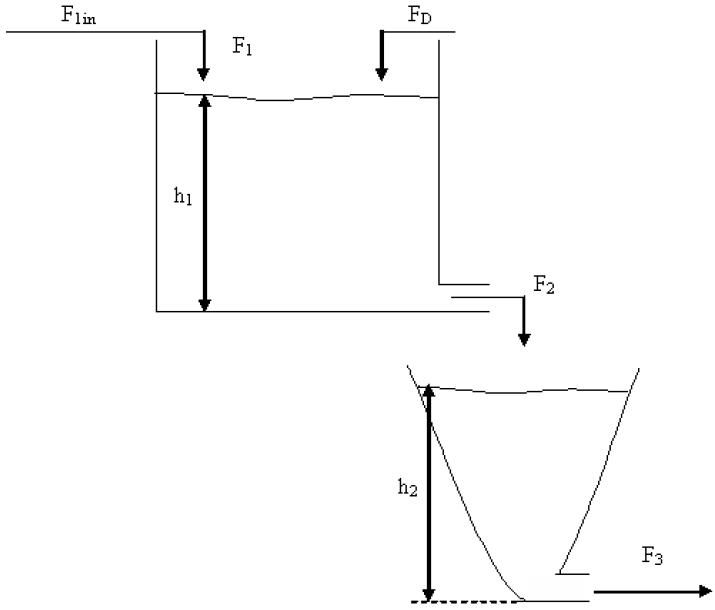
\includegraphics[width=0.8\textwidth]{pictures/schemat}
\caption{Obiekt regulacji automatycznej.}
\label{schemat}
\end{figure}

Wartością sterującą był dopływ $F_{1in}$ natomiast zakłóceniem - $F_D$. Z kolei wyjściem - wartością regulowaną - wysokość cieczy w drugim zbiorniku $h_2$. W pierwszej kolejności dokonano identyfikacji modelu, sprawdzono jego nieliniowość i dobrano odpowiedni rząd dynamiki modelu liniowego.
\section{Algorytmy regulacji predykcyjnej}
Do lat 70. ubiegłego wieku warstwa regulacji bezpośredniej w warstwowej strukturze sterowania (Rys. \ref{warstwy}) zapewniała przede wszystkim niezawodność \cite{120}. Dominowały wówczas algorytmy PID, natomiast rozwój optymalizacji postawił nowe wymagania przed układami regulacji \cite{160}. Okazało się bowiem, że skuteczna regulacja podczas optymalizacji punktu pracy przynosi duże korzyści ekonomiczne. To można było osiągnąć dzięki wprowadzeniu nowej grupy algorytmów - algorytmów regulacji predykcyjnej z przesuwnym horyzontem, zwanym też zasadą sterowania repetycyjnego \cite{160}. Pozwoliły po raz pierwszy rozwiązać problem uwzględnienia ograniczeń sygnałów sterujących.

\begin{figure}[h!]
\centering
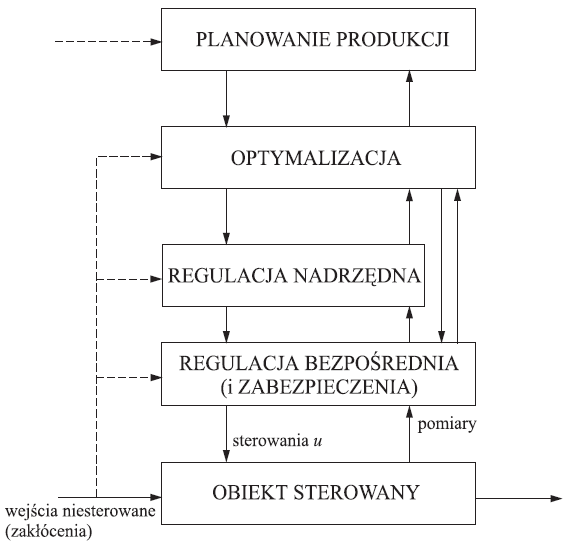
\includegraphics[width=0.5\textwidth]{pictures/warstwy}
\caption{Warstwowa struktura sterowania \cite{121}.}
\label{warstwy}
\end{figure}

W każdej chwili próbkowania, dysponując dynamicznym modele obiektu, pomiarami sygnałów procesowych oraz znaną lub założoną trajektorią wyjść zadanych wyznaczana jest sekwencja przyszłych wartości sygnału sterującego przez optymalizację funkcji celu zdefiniowanej na horyzoncie predykcji \cite{40}.

Najczęściej spotykana postać funkcji kryterialnej wygląda następująco:
\begin{equation}
J(k) = \min_{\Delta U(k)} \quad \{\sum_{p=1}^N (y^{zad}(k+p|k) - \hat{y}(k+p|k))^2 + \lambda \sum_{p=0}^{N_u} (\Delta u(k+p|k))^2\}
\end{equation}

przy ograniczeniach:

\begin{equation}
\begin{aligned}
u^{min} \quad &\leq& u(k+p|k) \quad &\leq& u^{max} \\
-\Delta u^{max} \quad &\leq& \Delta u(k+p|k) \quad &\leq& \Delta u^{max} \\
y^{min} \quad &\leq& \hat{y}(k+p|k) \quad &\leq& y^{max}
\end{aligned}
\end{equation}

\newpage

Wskaźnik jakości dostarcza informacji jakie wyniki powinien generować algorytm: uchyby regulacji muszą być jak najmniejsze, natomiast przyrosty sterowania nie powinny przyjmować dużych wartości, a ponadto korygowane są tzw. parametrem kary. Wyeliminowanie tego składnika ($\lambda = 0$) generuje przebiegi sygnału sterującego o dużych amplitudach i przyrostach, często niemożliwych do fizycznej realizacji. \\
Ograniczenia nałożone na sygnał sterujący związane są z uwarunkowaniami technologicznymi urządzeń wykonawczych, natomiast ograniczenia na sygnały wyjściowe służą spełnieniu norm technologicznych, ekonomicznych, a także zyskujących na coraz większym znaczeniu ekologicznych. Ogólna zasada regulacji predykcyjnej została zaprezentowana na Rys. \ref{mpc}

\begin{figure}[h!]
\centering
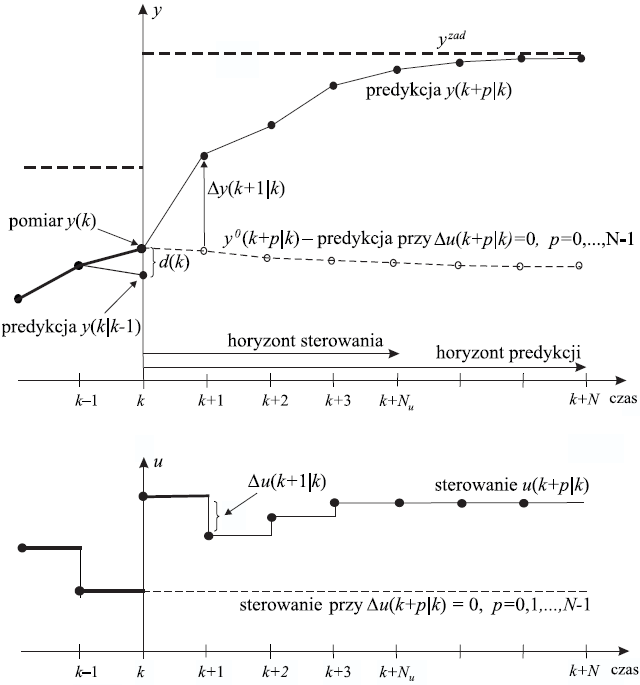
\includegraphics[width=0.65\textwidth]{pictures/mpc}
\caption{Zasada działania regulacji predykcyjnej \cite{122}.}
\label{mpc}
\end{figure}

Przedstawione przebiegi zawierają kilka istotnych aspektów, które warto opatrzeć komentarzem:
\begin{itemize}
\item[•] $y^{zad}$ - trajektoria sygnału zadanego, przyjmowana jako wartość stała na horyzoncie predykcji\footnote{Najczęściej zakładana jest stała trajektoria zadana, natomiast w niektórych dziedzinach, np. robotyka, dopuszcza się uwzględnienie zmian trajektorii zadanej w celu uprzedniego reagowania na jej zmiany.}
\item[•] $\Delta y(k+p|k)$ - prognozowana trajektoria odpowiedzi wymuszonej zależna tylko od zmiennych decyzyjnych - przyszłych przyrostów sterowań
\item[•] $y^0(k+p|k)$ - przewidywana odpowiedź swobodna, czyli wartości odpowiadające sytuacji, w której na całym horyzont predykcji $N$ utrzymywana byłaby wartość sterowania z chwili poprzedniej $u(k-1)$
\item[•] $\Delta u(k+p|k)$ - kolejne przyrosty sterowania wyznaczane na horyzoncie sterowania $N_u$
\end{itemize}

Na tej podstawie oraz korzystając z zasady superpozycji można zapisać:
\begin{equation}
y(k+p|k) = y^0(k+p|k) + \Delta y(k+p|k) \quad \quad p = 1 ... N
\end{equation}

\newpage

Zasada regulacji predykcyjnej jest dość uniwersalna co pozwoliło na wykształcenie kilku dominujących algorytmów, takich jak:
\begin{itemize}
\item[•] DMC (\textit{Dynamic Matrix Control}) - algorytm predykcyjny wykorzystujący model liniowy w postaci dyskretnych odpowiedzi skokowych
\item[•] GPC (\textit{Generalized Predictive Control}) - algorytm predykcyjny wykorzystujący model liniowy w postaci dyskretnych równań różnicowych
\item[•] MPCS (\textit{Model Predictive Control with State-space model}) - algorytm predykcyjny wykorzystujący w swoim opisie równania stanu
\item[•] MPHC (\textit{Model Predictive Heuristic Control}) - algorytm predykcyjny wykorzystujący model liniowy w postaci odpowiedzi impulsowej
\end{itemize}

Ze względu na praktyczną naturę algorytmu DMC do dalszych rozważań postanowiono przyjąć właśnie ten algorytm.

\section{Dynamic Matrix Control}
Algorytm DMC pierwszy raz został zaimplementowany przez grupę Shell Oil w latach \\ 70 XXw. Na tamten czas dało im to ogromną przewagę w branży petrochemicznej, a sam algorytm dzięki bezpośredniemu praktycznemu zastosowaniu stał się bardziej popularny. Algorytm ten zasadę swojego działania opiera na odpowiedzi skokowej, co wg autora \cite{120} stanowi jeden z najskuteczniejszych form identyfikacji obiektu. \\
Na Rys. \ref{step_response} przedstawiono przykład odpowiedzi skokowej na wymuszenie jednostkowe, zaprezentowane na horyzoncie dynamiki, czyli czas po którym wartość odpowiedzi skokowej można uznać za ustaloną, tj.
\begin{equation}
s_k = s_{k+1} = s_{k+2} = ... = s_D = s_{\infty}
\end{equation} 

\begin{figure}[h!]
\centering
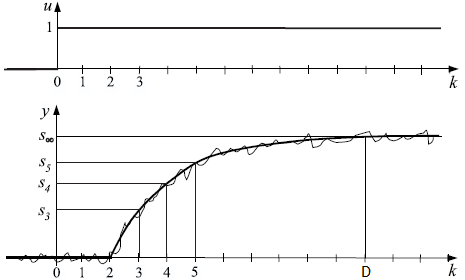
\includegraphics[width=0.75\textwidth]{pictures/step_response}
\caption{Odpowiedź skokowa \cite{123}.}
\label{step_response}
\end{figure}

Korzystając z zasady superpozycji, dla każdej chwili dyskretnej $k+p$, można zatem zapisać:

\begin{equation}
y^{mod}(k+p|k) = y^{mod}(0) + \sum_{j=1}^{k+p} s(j) \Delta u(k+p-j)
\end{equation}

\newpage

Z kolei wartość przewidywanej trajektorii wyjść można zapisać jako suma wartości modelu i~zakłócenia sprowadzonego do wyjścia:

\begin{equation}
\hat{y}(k+p|k) = y^{mod}(k+p|k) + d(k+p|k)
\end{equation} 

\noindent gdzie zakłócenie $d(k)$ jest równe różnicy między pomiarem wyjścia w chwili $k$, a wartością obliczoną z modelu w chwili $k-1$:

\begin{equation}
d(k) = y(k) - y^{mod}(k|k-1)
\end{equation}

\noindent natomiast ogólnie przejętą praktyką jest przyjmowanie modelu zakłóceń typu DMC, tj.

\begin{equation}
d(k+1|k) = d(k+2|k) = ... = d(k+N|k) = d(k)
\end{equation}

Takie założenia pozwalają na sformułowanie wyjściowej postaci trajektorii prognozowanej w algorytmie DMC:

\begin{equation}
\left\{
\begin{aligned}
\hat{y}(k+p|k) &= y^0(k+p|k) + \Delta y(k+p|k) \\
y^0(k+p|k) &= y(k) + \sum_{j=1}^k (s(j+p) - s(j))\Delta u(k-j)  \\
\Delta y(k+p|k) &= \sum_{j=1}^p s(j) \Delta u(k+p-j)
\end{aligned}
\right.
\label{prognoza}
\end{equation}

Zatem w ogólności można zapisać trajektoria prognozowana jest sumą odpowiedzi swobodnej i wymuszonej. Algorytm DMC występuje w wersji analitycznej bez oraz z rzutowaniem na ograniczenia oraz w wersji numerycznej, uwzględniającej te ograniczenia. 

\subsection{Algorytm DMC w wersji analitycznej}
Do sformułowania prawa regulacji w wersji analitycznej, w postaci wektorowej niezbędne jest zdefiniowanie wektorów postaci:

\begin{equation}
\begin{aligned}
Y^{zad} = \begin{bmatrix}
y^{zad}(k+1|k) \\ \vdots \\ y^{zad}(k+N|k)
\end{bmatrix}_{Nx1}, \quad
\hat{Y} = \begin{bmatrix}
\hat{y}(k+1|k) \\ \vdots \\ \hat{y}(k+N|k)
\end{bmatrix}_{Nx1}, \quad
\Delta U(k) = \begin{bmatrix}
\Delta u(k|k) \\ \vdots \\ \Delta u(k+N_u-1|k)
\end{bmatrix}_{N_ux1}
\end{aligned}
\end{equation}

\noindent Oraz macierzy wagowych:

\begin{equation}
\begin{aligned}
\Psi = \begin{bmatrix}
\psi_1 & & \\ & \ddots & \\ & & \psi_N
\end{bmatrix}_{NxN}, \quad
\Lambda = \begin{bmatrix}
\lambda_0 & & \\ & \ddots & \\ & & \lambda_{N_u-1}
\end{bmatrix}_{N_u x N_u}
\end{aligned}
\end{equation}

\noindent Tak zdefiniowane wektory pozwalają zapisać funkcję celu w postaci:

\begin{equation}
J(k) = \min_{\Delta U(k)} \{||Y^{zad} - \hat{Y}(k)||^2_\Psi + ||\Delta U(k)||^2_\Lambda \}
\label{cel}
\end{equation}

\noindent Odwołując się do równania \ref{prognoza} prognozowaną trajektorię wyjść w wersji macierzowo-wektorowej można zapisać w postaci:

\begin{equation}
\left\{
\begin{aligned}
\hat{Y} &= Y^0(k) + \Delta Y(k) \\
Y^0(k)& = Y(k) + M^P \Delta U^P(k) \\
\Delta Y(k) &= M \Delta U(k)
\end{aligned}
\right.
\end{equation}

\newpage

\noindent gdzie:
\begin{equation}
\begin{aligned}
&M^P = \begin{bmatrix}
s_2 - s_1 & s_3 - s_2 & \cdots & s_D - s_{D-1} \\
s_3 - s_1 & s_4 - s_2 & \cdots & s_D - s_{D-1} \\
\vdots & \vdots & \ddots & \vdots \\ 
s_{N+1} - s_1 & s_{N+2} - s_2 & \cdots & s_{N+D-1} - s_{D-1}
\end{bmatrix}_{Nx(D-1)} \\
&M = \begin{bmatrix}
s_1 & 0 & \cdots & 0 \\
s_2 & s_1 & \cdots & 0 \\ 
\vdots & \vdots & \ddots & \vdots \\
s_N & s_{N-1} & \cdots & s_{N-N_u+1} \\
\end{bmatrix}_{NxN_u}, \quad
\Delta U^P(k) = \begin{bmatrix}
\Delta u(k-1) \\ \vdots \\ \Delta u(k-D+1)
\end{bmatrix}_{(D-1)x1}
\end{aligned}
\end{equation}

\noindent Wektor $\Delta U^P(k)$ opisuje wartości przyrostów sterowań z poprzednich chwil, natomiast macierz $M$ nazywana jest macierzą dynamiczną. Uwzględniając postać funkcji kryterialnej (\ref{cel}) oraz przyjmując odpowiednie założenia $\Psi \geq 0$ oraz $\Lambda \geq 0$ wektor kolejnych przerostów sterowań dany jest wzorem:

\begin{equation}
\Delta U(k) = K(Y^{zad} - Y^0)
\label{delta_u}
\end{equation}

\noindent gdzie

\begin{equation}
K = (M^T \Psi M  + \Lambda)^{-1} M^T \Psi
\end{equation}

\noindent Zważywszy na fakt, że w każdej iteracji algorytmu wykorzystywany jest tylko pierwsza z wyznaczonych wartości przyrostów sterowań, równanie \ref{delta_u} można uprościć i zapisać w postaci:

\begin{equation}
\Delta u(k) = \bar{K_1} (Y^{zad} - Y^0(k))
\label{u_anal}
\end{equation}

\noindent gdzie $\bar{K_1}$ jest pierwszym wierszem macierzy $K$. Równanie \ref{u_anal} opisuje analityczną postać algorytmu DMC. Kolejnym istotnym aspektem jest rzutowanie wyznaczanych wartości na ograniczenia:

\begin{equation}
\begin{aligned}
u^{min} \quad &\leq& u(k+1|k) \quad &\leq& u^{max} \\
-\Delta u^{max} \quad &\leq& \Delta u(k|k) \quad &\leq& \Delta u^{max} \\
y^{min} \quad &\leq& \hat{y}(k|k) \quad &\leq& y^{max}
\end{aligned}
\end{equation}

Wersja analityczna DMC znajduje zastosowanie w praktyce, szczególnie w systemach liniowych o niewielkiej liczbie zmiennych sterowania i ograniczeń. Jednak w bardziej złożonych przypadkach, zwłaszcza z dużymi układami wielowymiarowymi lub w systemach nieliniowych, częściej stosuje się wersję numeryczną.

\subsection{Algorytm DMC w wersji numerycznej}
Kwadratowa funkcja kryterialna - dzięki zastosowaniu modelu liniowego do predykcji - umożliwia rozwiązanie zadania minimalizacji w sposób analityczny, ale również numeryczny. Optymalizacja numeryczna ma tę przewagę, że pozwala uwzględnić ograniczenia nałożone na sygnał sterujący \cite{160}, tzn. w każdej iteracji wyznaczany jest wektor przyszłych sterowań w wyniku rozwiązania następującego zadania optymalizacji w postaci standardowej:

\begin{equation}
min \{J(x) = \frac{1}{2} x^T Hx + f^T x\} \\
\end{equation} 

\noindent przy ograniczeniach:

\begin{equation}
\begin{aligned}
x_{min} \leq &x \leq x_{max} \\
Ax &\leq b
\end{aligned}
\end{equation}

\newpage

\noindent gdzie:

\begin{equation}
\begin{aligned}
x &= \Delta U(k), \quad x_{min} = -\Delta U_{max}, \quad x_max = \Delta U_max \\
H &= 2(M^T \Psi M + \Lambda) \\
f &= -2M^T \Psi (Y^{zad}(k) - Y^0(k)) \\
A &= \begin{bmatrix}
-J \\ J \\ -M \\ M
\end{bmatrix}, \quad
b = \begin{bmatrix}
-U_{min} + U(k-1) \\ U_{max} - U(k-1) \\ 
-Y_{min} + Y^0(k) \\ Y_{max} - Y^0(k) 	 	
\end{bmatrix} \\
J &= \mathbb{I}_{N_u x N_u}, \quad Y_{min} = [y_{min}, ..., y_{min}]^T, \quad Y_{max} = [y_{max}, ..., y_{max}]^T
\end{aligned}
\end{equation}

Działanie regulatora DMC z ograniczeniami zostało przedstawione w pracy \cite{50}, w której autorzy dokonali szereg testów sprawdzających wpływ przeprowadzanej optymalizacji w każdym kroku na jakość regulacji.

\subsection{Inne warianty DMC}
Zastosowanie algorytmów predykcyjnych w latach 70. ubiegłego stulecia pokazało jak duże korzyści - nie tylko w aspekcie jakości regulacji, ale także ekonomicznych - może przynieść ich wdrożenie do obiektu sterowania. Wówczas ten fakt spowodował dynamiczny rozwój tych algorytmów, czego efektem są m.in. algorytmy wykorzystujące nieliniowe modele obiektów:
\begin{itemize}
\item[-] Algorytm DMC z sukcesywną linearyzacją (DMC-SL)
\item[-] Algorytm DMC z nieliniową optymalizacją (DMC-NO)
\item[-] Algorytm DMC z nieliniową predykcją i linearyzacją (DMC-NPL)
\end{itemize}

\begin{description}
\item \textbf{DMC-SL} \\
Algorytm podstawowy, korzystający z modelu liniowego często może okazać się niewystarczający, np. gdy obiekt wykazuje silną nieliniowość. Dużą poprawę, tj. minimalizację błędów linearyzacji, można osiągnąć implementując algorytm predykcyjny z sukcesywną linearyzacją. W każdej iteracji, dokonywana jest linearyzacja modelu nieliniowego w punkcie pracy, w którym aktualnie znajduje się obiekt. Następnie na podstawie modelu liniowego wyznaczana jest odpowiedź skokowa oraz formowana jest macierz dynamiczna \cite{170, 120}. Okazuje się, że linearyzacja modelu nie jest wymagana w każdym kroku, co zaprezentował autor \cite{30}. Jeśli zmiany między kolejnymi wartościami predykcji nie są duże, można korzystać z uprzednio wyznaczonego modelu liniowego.

\item \textbf{DMC-NPL} \\
Algorytm DMC z nieliniową predykcją i linearyzacją jest zmodyfikowaną wersją algorytmu wykorzystującą sukcesywną linearyzacji. W tym przypadku bowiem odpowiedź swobodna jest wyznaczana na podstawie modelu nieliniowego, natomiast linearyzacja służy wyznaczeniu odpowiedzi skokowej i sformułowania macierzy dynamicznej - podobnie jak w DMC-SL. Marginalizacja wpływu modelu liniowego na proces przynosi poprawę szczególnie w przypadkach gdy regulowany obiekt wykazuję silną nieliniowość charakteryzuje się szybkim przechodzenie do odległych punktów równowagi, np. po wystąpieniu silnych zakłóceń czy tez przy uruchamianiu lub wyłączaniu procesów \cite{170, 120}.

\item \textbf{DMC-NO} \\
Algorytm ten zaliczany jest do grupy algorytmów z nieliniową optymalizacją. Wykorzystuje pełny nieliniowy model procesu do predykcji. Prostota koncepcji i jakość regulacji na najwyższym poziomie nie są jednak w stanie zrekompensować istotnych wad tego podejścia, mianowicie złożoność obliczeniowa oraz fakt, że nie istnieją algorytmy rozwiązujące nieliniowy problem optymalizacji w możliwym do oszacowania czasie eliminują algorytm DMC-NO z praktycznego użycia \cite{170}.
\end{description}
\chapter{Regulacja rozmyta}
Tytułowy typ regulacji zrywa ze standardową procedurą podejmowania decyzji w sposób binarny, tzn. $1 / 0$ \cite{40}. Na Rys. \ref{crisp} przedstawiono standardową funkcję przynależności do zbioru, którą można opisać wzorem:

\begin{equation}
\mu_C = \begin{cases}
1, \quad x \in [a, b] \\
0, \quad x \notin [a, b]
\end{cases}
\end{equation}

\begin{figure}[h!]
\centering
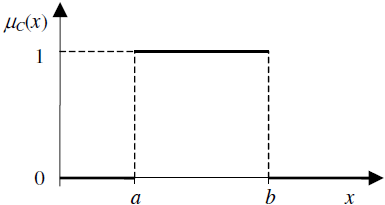
\includegraphics[width=0.5\textwidth]{pictures/crisp}
\caption{Funkcja przynależności zbioru ostrego.}
\label{crisp}
\end{figure}

Natomiast istota wnioskowania rozmytego polega na zgromadzeniu wiedzy eksperckiej, operatora procesu, wspartej odpowiedzią skokową obiektu, które pozwolą na sformułowanie zbiorów rozmytych (Rys. \ref{fuzzy_set}) oraz bazy reguł definiującej regulator rozmyty \cite{160, 170}. Funkcja przynależności zbioru rozmytego została zaprezentowana na Rys. \ref{fuzzy} i w tym przypadku dana jest wzorem:

\begin{equation}
\mu_C = \begin{cases}
0,& \quad x \leq c \vee x \geq f \\
\frac{x-c}{d-c},& \quad c \leq x \leq d \\ 
1,& \quad d \leq x \leq e \\
\frac{f-x}{f-e},& \quad e \leq x \leq f
\end{cases}
\end{equation}

\begin{figure}[h!]
\centering
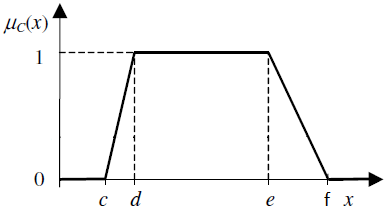
\includegraphics[width=0.5\textwidth]{pictures/fuzzy}
\caption{Funkcja przynależności zbioru rozmytego.}
\label{fuzzy}
\end{figure}

\newpage

\noindent Zmienne z odcinków $[c,d]$ oraz $[e,f]$ przyjmują wartości z przedziału $[0,1]$, w tym sensie granice zbioru przynależności są rozmyte. Natomiast wartość funkcji przynależności do zbioru określana jest stopniem przynależności. Należy w tym miejscu zwrócić uwagę na kształty funkcji przynależności. Funkcje trapezowe bądź trójkątne proste w swym zapisie, nie są różniczkowalne. Aspekt ten jest o tyle istotny, że zapewnia stabilność, zwiększa dokładność w systemach sterowania rozmytego, a także jest niezbędny podczas uczenia maszynowego, wykorzystującego metody gradientowe. Dlatego w wielu zastosowaniach przyjęło się korzystanie z innych kształtów funkcji przynależności, zapewniających różniczkowalność, takich jak: gaussowskie, dzwonowe, sigmoidalne.

\begin{figure}[h!]
\centering
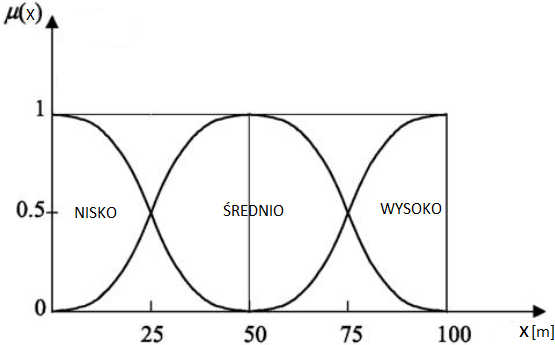
\includegraphics[width=0.75\textwidth]{pictures/fuzzy_set}
\caption{Przykładowe zbiory rozmyte.}
\label{fuzzy_set}
\end{figure}

Ważną kwestią w rozumieniu systemów rozmytych, jest pośrednik między zmienną numeryczną, a zmienną symboliczną - zmienna lingwistyczna. Na Rys. \ref{fuzzy_set} przedstawiono rozmycie zmiennej "wysokość", która przyjmuje trzy wartości: "nisko", "średnio", "wysoko" i tak można zauważyć, że wartość numeryczna $75m$ ze stopniem przynależności $0,5$ należy do zbiorów "średnio" oraz "wysoko" \cite{90, 120, 130}. \\
Po rozmyciu zmiennej lingwistycznej, określeniu stopni przynależności danych wartości do poszczególnych zbiorów pozostaje jeszcze zdefiniowanie bazy wiedzy, czyli tzw. zbioru reguł. Każda reguła składa się z części warunkowej, zwanej poprzednikiem oraz konsekwencji, określanej następnikiem. Ogólna struktura reguły w rozumieniu systemów rozmytych przyjmuje postać:

\begin{equation}
\text{JEŚLI } <poprzednik> \text{ TO } <następnik> 
\end{equation}

Poprzedniki reguł w najprostszym przypadku mogą zawierać pojedynczy warunek w innej sytuacji mogą składać się z kilku prostych warunków połączonych operacjami logicznymi (i, lub, nie).

\begin{itemize}
\item[•] warunek prosty: $\text{JEŚLI } x \text{ jest } A \text{ TO } <następnik>$ \\
\item[•] warunek złożony: $\text{JEŚLI } x_1 \text{ jest } A_1 \text{ lub } x_2 \text{ jest } A_2 \text{ i } x_3 \text{ nie jest } A_3 \text{ TO } <następnik>$ \\
\end{itemize}

\newpage

W przypadku następników reguł wyróżnić można ich trzy postaci:

\begin{enumerate}
\item Następnik ostry
\begin{equation}
\text{JEŚLI } <poprzednik> \text{ TO } y = y_a
\end{equation}

\item Następnik rozmyty 
\begin{equation}
\text{JEŚLI } <poprzednik> \text{ TO } y \text{ jest } Y_a
\end{equation}

\item Następnik funkcyjny
\begin{equation}
\text{JEŚLI } <poprzednik> \text{ TO } y = f(x_1, x_2, ... , x_k)
\end{equation}
\end{enumerate}

\noindent Szczególnie istotne oraz wykorzystywane w praktyce są dwie ostatnie wymienione metody. Następniki w postaci zbiorów rozmytych są z powodzeniem wykorzystywane w modelach Mamdaniego \cite{170, 90}, gdzie wykorzystując wiedzę eksperta można z dużą dokładnością sterować obiektem regulacji w sposób rozmyty. Częstą praktyką w tym podejściu jest budowanie tablicy decyzyjnej, która w stosunkowo prosty i przejrzysty sposób redukuję bazę reguł do tabeli \cite{170}. \\
W kontekście niniejszej pracy skupiono się przede wszystkim na następnikach funkcyjnych opisujących modele Takagi - Sugeno, którym poświęcono następny rozdział. 

\section{Modele Takagi-Sugeno}
Projektowanie modeli Takagi-Sugeno składa się z następujących etapów:

\begin{enumerate}
\item Obliczenie poziomów aktywacji reguł
\item Wyznaczenie konkluzji - obliczenie wartości następników funkcyjnych poszczególnych reguł
\item Wyznaczenie konkluzji końcowej - zsumowanie wartości następników funkcyjnych - ważone i normowane - z uwzględnieniem sił odpalenia reguł, co opisuje wzór \ref{wniosek}.
\end{enumerate}

\begin{equation}
y = \frac{\sum_{j=1}^r w^j y^j}{\sum_{j=1}^r w^j}
\label{wniosek}
\end{equation}

\noindent gdzie:
\begin{itemize}
\item[•] $r$ - liczba reguł
\item[•] $w^j$ - siły odpalenia poszczególnych reguł
\item[•] $y^j$ - wartości odpowiednich następników funkcyjnych
\end{itemize}

Ogólnie modele rozmyte służą do aproksymacji funkcji nieliniowych stąd w przypadku modeli Takagi-Sugeno następniki funkcyjne występują najczęściej w postaci funkcji wielomianowych pierwszego rzędu \cite{160, 170}:

\begin{equation}
\text{JEŚLI } <poprzednik> \text{ TO } y = a_0 + \sum_{j=1}^n a_jx_j
\end{equation} 

Natomiast w pracy skupiono się jakie korzyści może przynieść zastosowanie nieliniowych - hiperbolicznych - następników. Według autorów \cite{80} pozwala to na zmniejszenie liczby zbiorów rozmytych, a tym samym reguł.

\newpage

\section{Podejście PDC}
Podejście PDC (\textit{Parallel Distributed Combensation}) zakłada dedukcję regulatora za pomocą modelu Takagi-Sugeno obiektu. Istota równoległej kompensacji rozproszonej polega na dobraniu dla każdego następnika rozmytego lokalnego regulatora liniowego. Zatem w wyniku takiego podejścia otrzymuje się tyle regulatorów z ilu modeli lokalnych, opisujących obiekt w danych obszarze, składa się system rozmyty. Na początku zakłada się taką samą postać poprzedników jak w modelu obiektu, następnie w miarę potrzeby dostraja \cite{120, 170}. Struktura regulatora otrzymanego w wyniku zastosowania podejścia PDC została przedstawiona na Rys. \ref{pdc}.

\begin{figure}[h!]
\centering
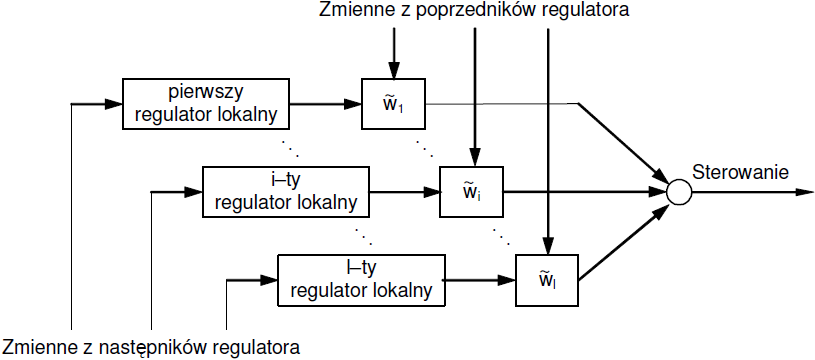
\includegraphics[width=0.75\textwidth]{pictures/pdc}
\caption{Struktura regulatora rozmytego otrzymanego podejściem PDC \cite{171}.}
\label{pdc}
\end{figure}
\chapter{Modele Hammersteina i Wienera}
Istotą stosowania modeli Hammersteina i Wienera jest rozdzielenie liniowej dynamiki od zakłóceń wprowadzanych przez statyczne nieliniowości. Mogę one występować na wejściu \\ (Rys. \ref{hamm}) bądź wyjściu (Rys. \ref{wien}) \cite{10}.
\vspace{0.5cm}
\begin{figure}[h!]
\centering
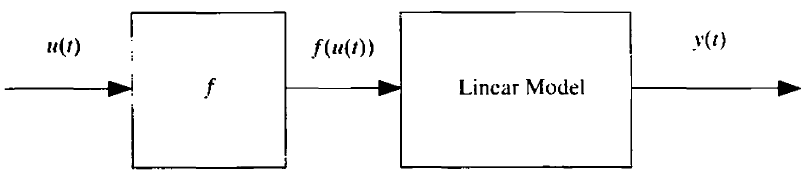
\includegraphics[width=\textwidth]{pictures/hammerstein}
\caption{Model Hammersteina \cite{21}.}
\label{hamm}

\vspace{0.5cm}

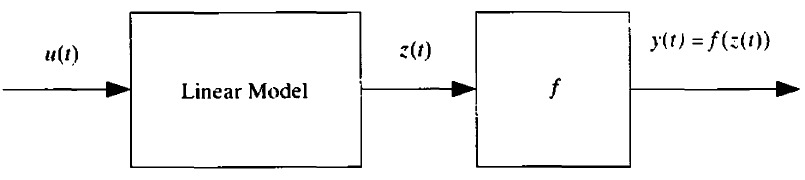
\includegraphics[width=\textwidth]{pictures/wiener}
\caption{Model Wienera \cite{21}.}
\label{wien}
\end{figure}

Modele te doskonale nadają się do identyfikacji systemów nieliniowych. Często w tym celu wykorzystywane są funkcje wielomianowe, sieci neuronowe czy systemy rozmyte \cite{150}.

\chapter{Wstęp}
Praca zawiera porównanie modeli Hammersteina oraz Wienera w regulacji kaskadowej. Bazą porównania był obiekt opisany równaniami fizycznymi postaci:
\begin{equation}
\begin{cases}
\frac{dV_1}{dt} = F_1 + F_D - F_2(h_1) \\
\frac{dV_2}{dt} = F_2(h_1) - F_3(h_2) \\
F_2(h_1) = \alpha_1 \sqrt{h_1}, \quad F_3(h_2) = \alpha_2 \sqrt{h_2}, \quad V_1(h_1) = A_1h_1, \quad V_2(h_2) = C_2h_2^2, \quad F_1(t) = F_{1in}(t-\tau)  
\end{cases}
\label{model_fiz}
\end{equation}

\begin{itemize}
\item[•] Stałe: 
\begin{equation}
A_1 = 540cm^2, \quad C_2 = \num{0.85}, \quad \alpha_1 = 26, \quad \alpha_2 = 20
\end{equation}

\item[•] Punkt pracy:
\begin{equation}
F_1 = 90 \frac{cm^3}{s}, \quad F_D = 30 \frac{cm^3}{s}, \quad \tau = 100, \quad h_2 = 36cm
\end{equation}
\end{itemize}

\noindent gdzie użyte oznaczenia odpowiadają tym zastosowanym na rys. \ref{schemat}.

\begin{figure}[h!]
\centering
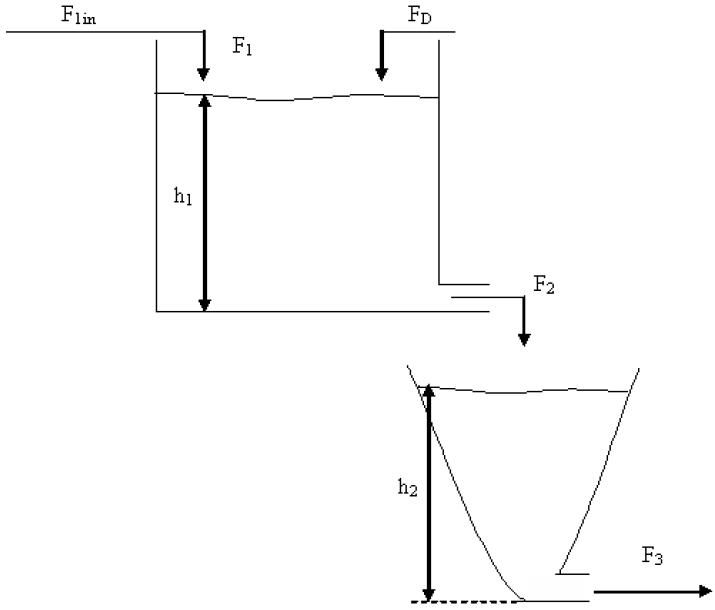
\includegraphics[width=0.8\textwidth]{pictures/schemat}
\caption{Obiekt regulacji automatycznej.}
\label{schemat}
\end{figure}

Wartością sterującą był dopływ $F_{1in}$ natomiast zakłóceniem - $F_D$. Z kolei wyjściem - wartością regulowaną - wysokość cieczy w drugim zbiorniku $h_2$. W pierwszej kolejności dokonano identyfikacji modelu, sprawdzono jego nieliniowość i dobrano odpowiedni rząd dynamiki modelu liniowego.
\chapter{Identyfikacja}
\section{Charakterystyka statyczna}
Poświęcono jej bardzo dużo uwagi, ze względu na kluczową rolę, jaką odgrywa we wspomnianych modelach Hammersteina i Wienera. Korzystając z modelu fizycznego, z równania \ref{model_fiz} wyznaczono:
\begin{equation}
\frac{dV_1}{dt} = 0 \quad \wedge \quad \frac{dV_2}{dt} = 0
\end{equation}

\noindent wobec tego:
\begin{equation}
\begin{cases}
F_1 + F_D - \alpha_1 \sqrt{h_1} &= 0 \\
\alpha_1 \sqrt{h_1} - \alpha_2 \sqrt{h_2} &= 0
\end{cases}
\end{equation}

\noindent Po prostych przekształceniach otrzymano wzór opisujący charakterystykę statyczną:
\begin{equation}
h_2 = \left( \frac{F_1 + F_D}{\alpha_2} \right)^2
\end{equation}

\noindent Wykres odpowiadający wyprowadzonemu wzorowi prezentuje się następująco:

\begin{figure}[h!]
\centering
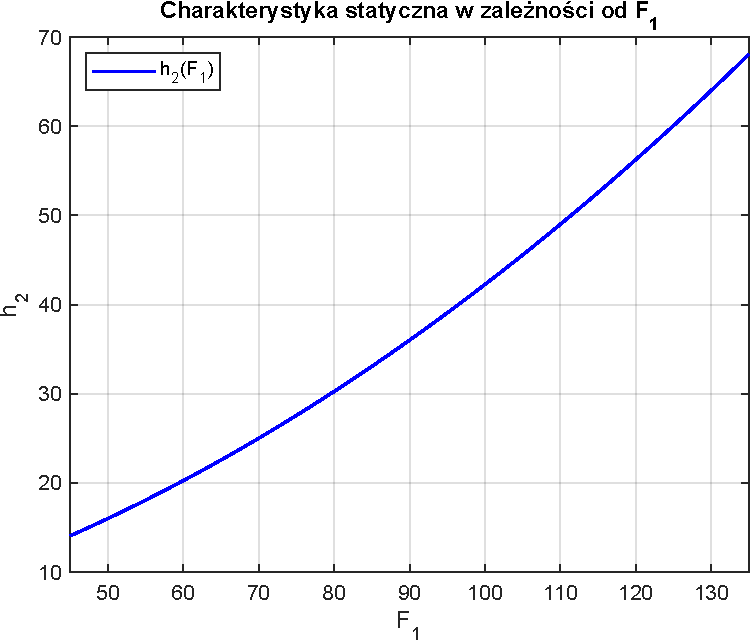
\includegraphics[width=0.8\textwidth]{pictures/static_characteristic}
\caption{Charakterystyka statyczna $h_2(F_1)$.}
\label{static_characteristic}
\end{figure}

\noindent Założono przedział zmienności sygnału sterującego w zakresie $F_1 \in [-45, 45]$.

\newpage

\section{Wymuszenia}
Po dokonaniu pierwszego kroku identyfikacji - wykreślenia charakterystyki statycznej - uzyskano wstępne informacje o obiekcie. Równania opisujące model (\ref{model_fiz}) oraz charakterystyka statyczna przedstawiona na rys. \ref{static_characteristic} pokazuje, że obiekt jest nieliniowy, stąd dokonano jego linearyzacji w punkcie pracy, tj.:
\begin{equation}
\begin{cases}
\frac{dV_1}{dt} \cong F_1 + F_D - \alpha_1 \sqrt{\frac{V_{10}}{A}} - \frac{\alpha_1}{2 \sqrt{A \cdot V_{10}}} \cdot (V_1 - V_{10})\\
\frac{dV_2}{dt} \cong \alpha_1 \sqrt{\frac{V_{10}}{A}} - \alpha_2 \sqrt[4]{\frac{V_{20}}{C}} + \frac{\alpha_1}{2 \sqrt{A \cdot V_{10}}} \cdot (V_1 - V_{10}) - \frac{\alpha_2}{4 \sqrt[4]{C \cdot V_{20}^3}} \cdot (V_2 - V_{20})
\end{cases}
\end{equation}

\noindent Linearyzacji dokonano przyjmując jako zmienną stanu objętość cieczy w obu zbiornikach. 

\begin{equation}
x = \begin{bmatrix} V_1 & V_2 \end{bmatrix}^T
\end{equation}

Następnie, podając wygenerowaną sekwencję sygnału sterującego, zbadano rozbieżność modelu liniowego i nieliniowego.

\begin{figure}[h!]
\centering
\subfloat[Wygenerowana sekwencja sygnału sterującego $u(k)$.]{
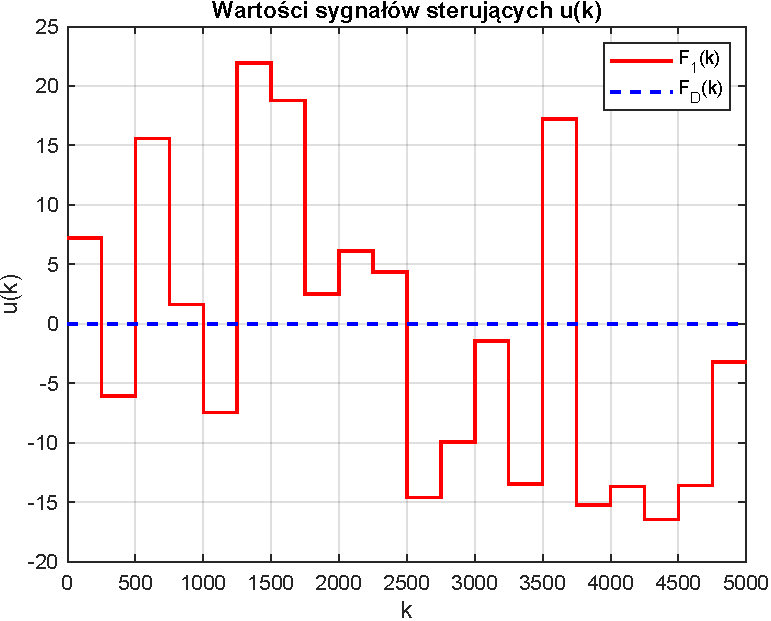
\includegraphics[width=0.45\textwidth]{pictures/u_F1}}
\hfill
\subfloat[Sygnał wyjściowy $y(k)$.]{
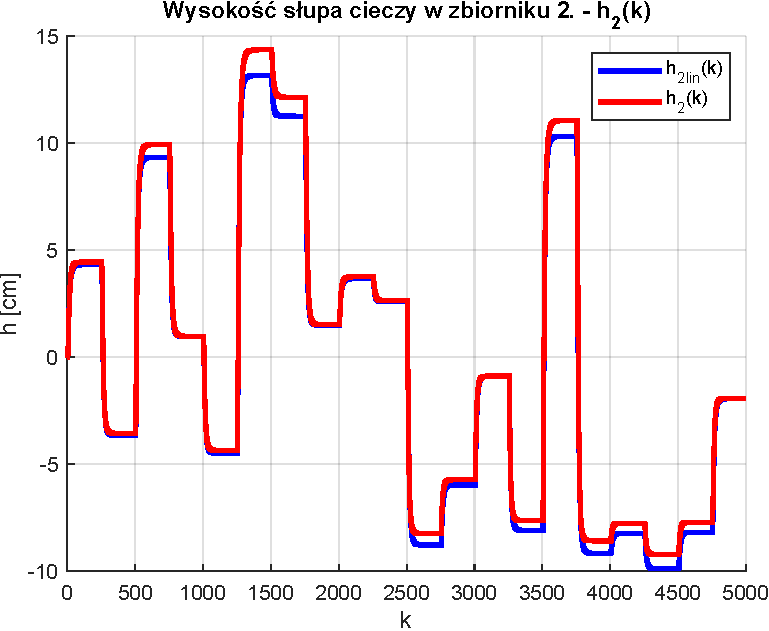
\includegraphics[width=0.45\textwidth]{pictures/y_F1}}
\caption{Porównanie modelu liniowego z nieliniowym.}
\end{figure}

Otrzymano dokładnie to czego się spodziewano. Wymuszenia nie większe niż $\pm 10 \frac{cm^3}{s}$ nie powodują znacznego wytrącenia układu z położenia równowagi, dzięki czemu model liniowy bardzo dobrze aproksymuje zachowanie układu. Niestety sytuacja pogarsza się wraz z oddalaniem się od punktu pracy - model liniowy zaczyna poważnie odbiegać od modelu nieliniowego, opisującego obiekt. W celach porównawczych policzono błędy, testując model w trybie bez rekurencji (ARX) oraz z rekurencją OE, przyjmując jako kryterium jakości błąd średni kwadratowy, tj.:

\begin{equation}
E = \sum_{k=0}^N (y(k) - y^{mod}(k))^2
\end{equation}

\noindent Wcześniej dokonano podziału wygenerowanych danych dynamicznych na dwa zbiory - uczący i~weryfikujący - stosując zasadę podziału $0\% - 50\% / 50\% - 100\%$, potrzebne do późniejszego, ewentualnego dostrajania modelu. Otrzymano następujące wyniki:

\begin{description}
\item[ARX] 
\begin{equation}
E_{ucz} = \num{0.002} \hspace{1cm} E_{wer}=\num{0.003}
\end{equation}
\item[OE] 
\begin{equation}
E_{ucz} = \num{0.470} \hspace{1cm} E_{wer}=\num{0.831}
\end{equation}
\end{description}

%\newpage

\begin{figure}[p!]
\begin{center}
\Large \textbf{Model ARX}
\end{center} 
\centering
\subfloat[Zbiór uczący.]{
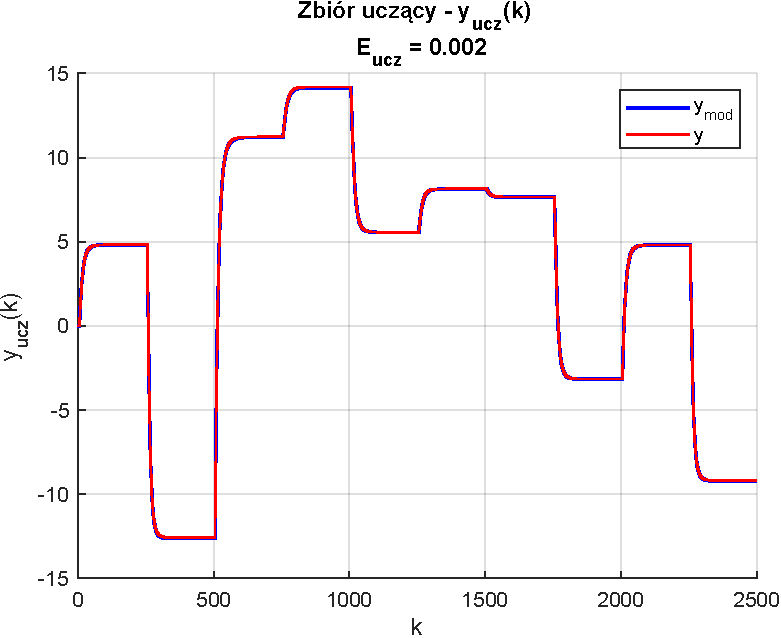
\includegraphics[width=0.45\textwidth]{pictures/arx_ucz}}
\hfill
\subfloat[Zbiór weryfikujący.]{
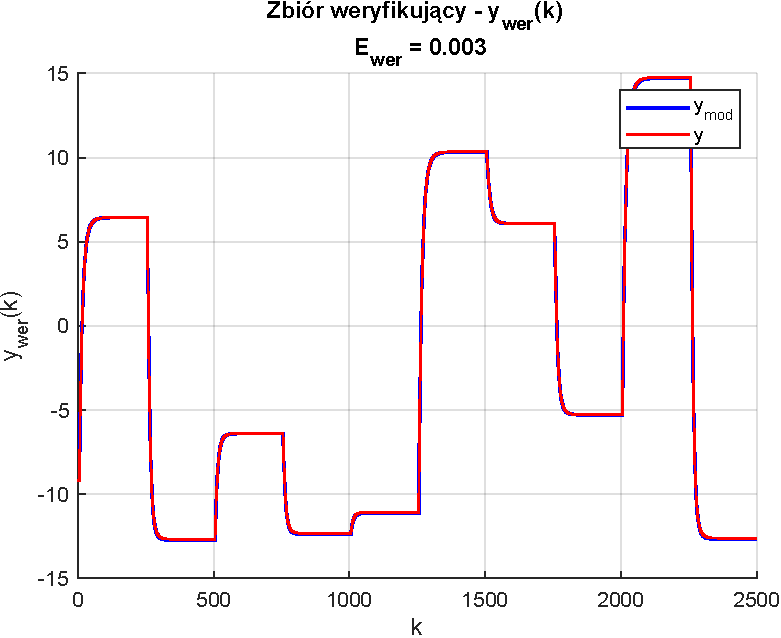
\includegraphics[width=0.45\textwidth]{pictures/arx_wer}}

\begin{center}
\Large \textbf{Model OE}
\end{center} 
\subfloat[Zbiór uczący.]{
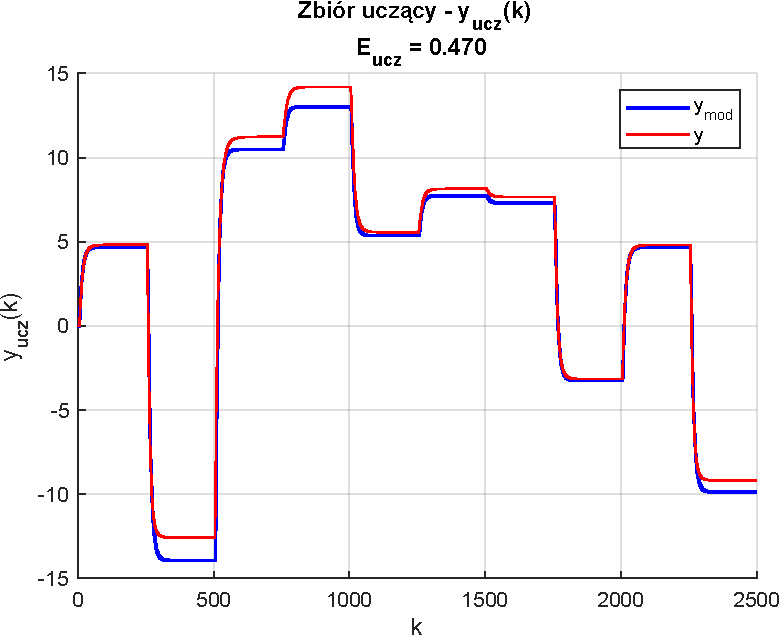
\includegraphics[width=0.45\textwidth]{pictures/oe_ucz}}
\hfill
\subfloat[Zbiór weryfikujący.]{
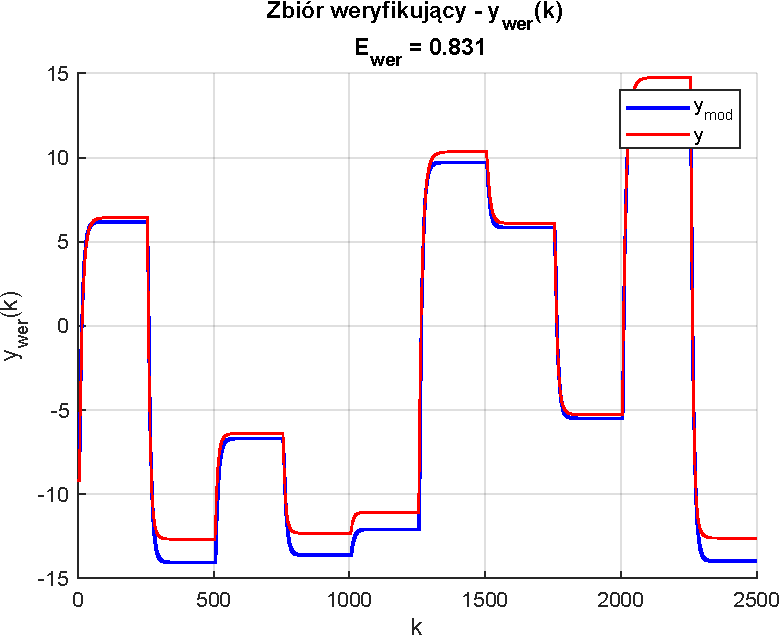
\includegraphics[width=0.45\textwidth]{pictures/oe_wer}}
\caption{Symulacja odpowiednich modeli z wykorzystaniem wygenerowanej sekwencji sygnału sterującego.}
\end{figure}

\newpage

\section{Podejście inżynierskie}
Od tej pory do dalszej analizy postanowiono przyjąć model szarej skrzynki. Informacją o obiekcie był fakt, że układ był inercyjny. Zadano więc wymuszenie w postaci skoku jednostkowego i starano się aproksymować odpowiedź układu dobierając odpowiednie parametru dla modelu transmitancji \textit{First Order Plus Dead Time} (FOPDT), który wyraża się wzorem:

\begin{equation}
G(s) = \frac{K_0e^{-sT_0}}{T_1s + 1}
\end{equation}

\noindent Dobrane parametry:

\begin{equation}
K_0 = \num{0.6025} \hspace{1cm} T_0 = 100 \hspace{1cm} T_1 = 225
\end{equation}

\begin{figure}[h!]
\centering
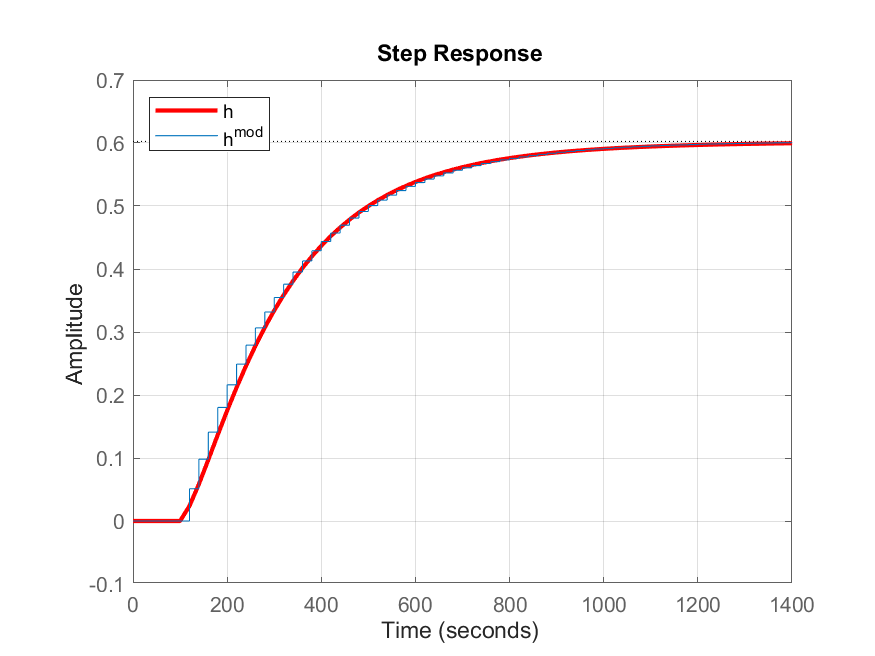
\includegraphics[width=\textwidth]{pictures/model_fopdt}
\caption{Aproksymacja odpowiedzi skokowej układu modelem FOPDT.}
\end{figure}

\newpage

Uzyskany rezultat nie był satysfakcjonujący stąd przyjęto model \textit{Second Order Plus Dead Time} (SOPDT), tj.

\begin{equation}
G(s) = \frac{K_0e^{-sT_0}}{(T_1s + 1)(T_2s + 1)}
\end{equation}

\noindent Dobrane parametry:

\begin{equation}
K_0 = \num{0.6025} \hspace{1cm} T_0 = 100 \hspace{1cm} T_1 = 212 \hspace{1cm} T_2 = 15
\end{equation}

\noindent Wynik prezentował się następująco:

\begin{figure}[h!]
\centering
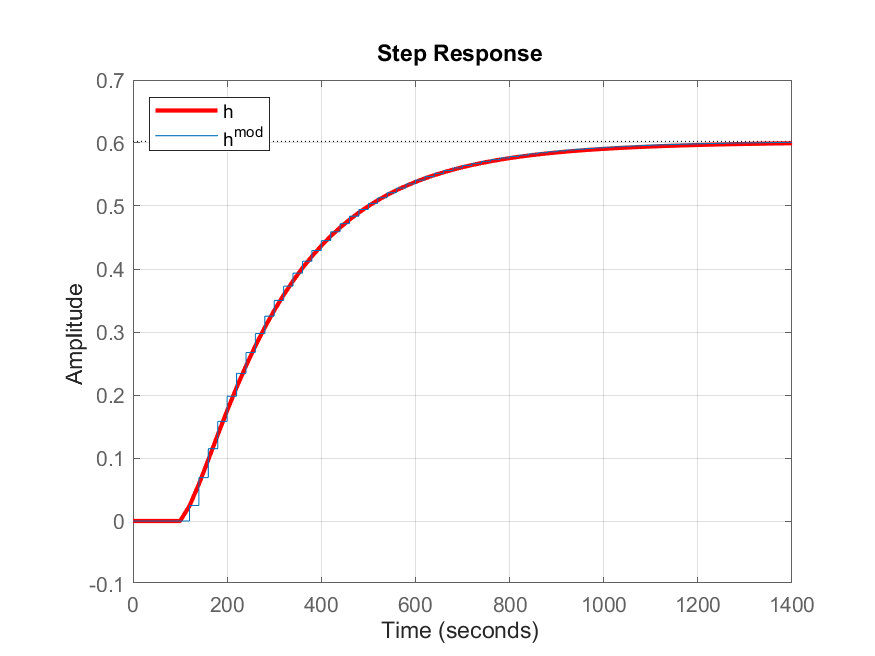
\includegraphics[width=\textwidth]{pictures/model_sopdt}
\caption{Aproksymacja odpowiedzi skokowej układu modelem SOPDT.}
\end{figure}

\newpage

Ponownie, chcąc sprawdzić skuteczność aproksymacji obiektu regulacji wygenerowanym modelem, którego równanie różnicowe jest postaci:

\begin{equation}
\begin{aligned}
y(k) = \num{1.174} y(k-1) - \num{0.2399} y(k-2) + &\num{0.02459} u_1(k-6) + \num{0.01536} u_1(k-7) \\ 
+&\num{0.02459} u_2(k-1) + \num{0.01536} u_2(k-2) 
\end{aligned}
\label{diff_eq}
\end{equation}

\noindent wygenerowano sekwencję sygnału sterującego $u_1(k)$ oraz $u_2(k)$, który są przyrostami wartości sterujących odpowiednio $F_1$ oraz $F_D$.

\begin{figure}[h!]
\begin{center}
\Large \textbf{Model ARX}
\end{center} 
\centering
\subfloat[Zbiór uczący.]{
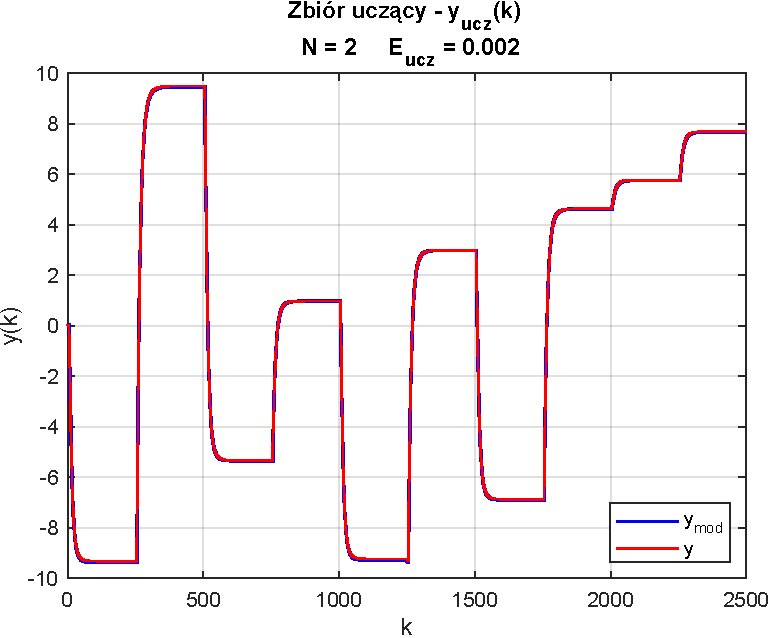
\includegraphics[width=0.45\textwidth]{pictures/arx_ucz_sopdt}}
\hfill
\subfloat[Zbiór weryfikujący.]{
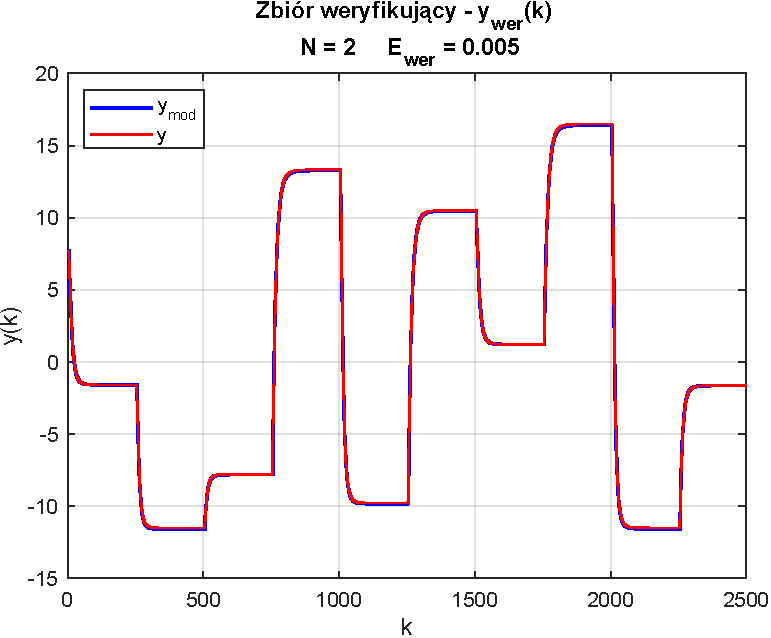
\includegraphics[width=0.45\textwidth]{pictures/arx_wer_sopdt}}

\begin{center}
\Large \textbf{Model OE}
\end{center} 
\subfloat[Zbiór uczący.]{
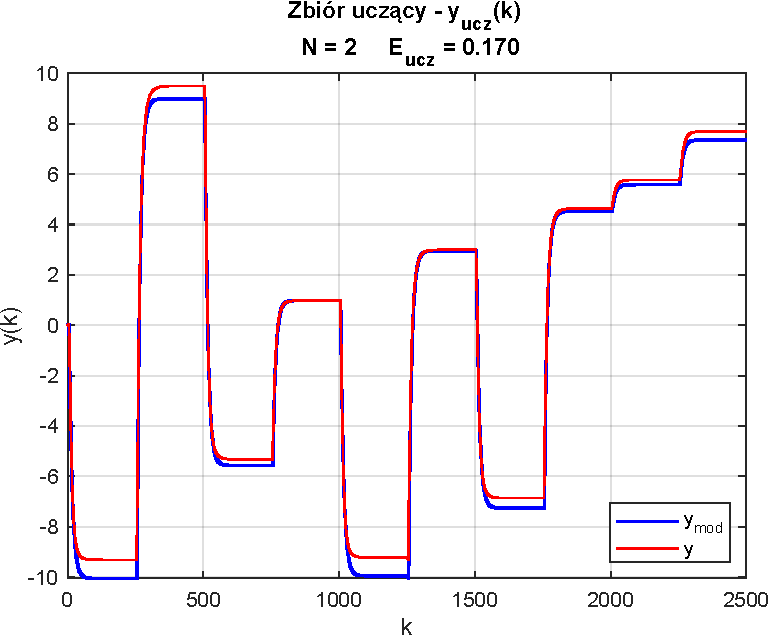
\includegraphics[width=0.45\textwidth]{pictures/oe_ucz_sopdt}}
\hfill
\subfloat[Zbiór weryfikujący.]{
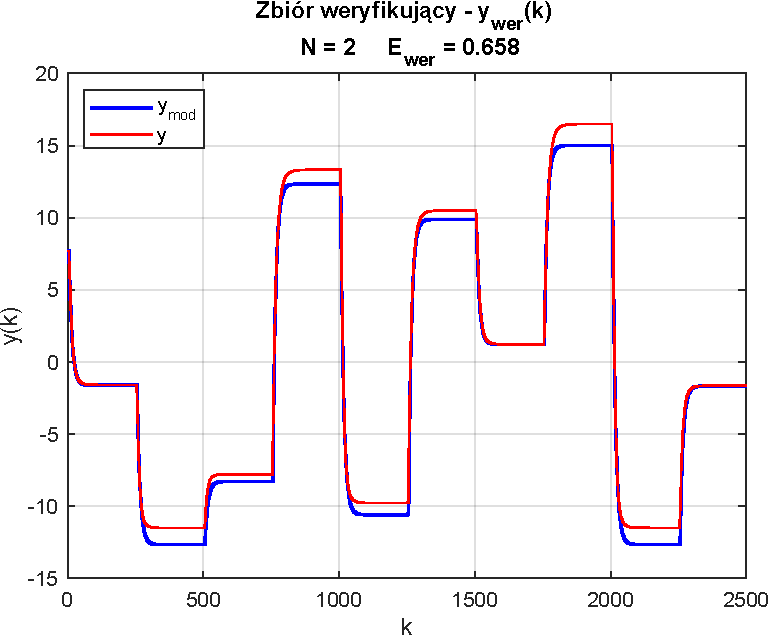
\includegraphics[width=0.45\textwidth]{pictures/oe_wer_sopdt}}
\caption{Symulacja odpowiednich modeli z wykorzystaniem wygenerowanej sekwencji sygnału sterującego.}
\end{figure}

Błędy uznano za akceptowalne na tym poziomie identyfikacji i przyjęto wyznaczony model do dalszej analizy.
\section{Model Hammersteina}
Po przeanalizowaniu charakterystyki statycznej oraz porównaniu modelu nieliniowego z liniowym przystąpiono do identyfikacji modelu Hammersteina.
Istota polega na umieszczeniu nieliniowego bloku statycznego przed liniowym blokiem dynamicznym, co pozwala na oddzielenie nieliniowości od dynamiki systemu. Jego główną zaletą jest prostsza identyfikacja parametrów, ponieważ najpierw określa się charakterystykę statyczną, a dopiero potem analizuje dynamikę. Takie podejście lepiej odwzorowuje systemy, w których nieliniowości wynikają z właściwości aktuatorów lub czujników, a część dynamiczna pozostaje liniowa. Graficzne ujęcie opisanego modelu zilustrowano na rys. \ref{hamm_model}.

\begin{figure}[h!]
\centering
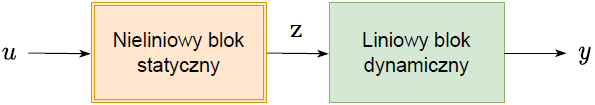
\includegraphics[width=\textwidth]{pictures/hamm_model}
\caption{Reprezentacja graficzna modelu Hammersteina.}
\label{hamm_model}
\end{figure}

\noindent Cała procedura w przypadku analizowanego obiektu wygląda następująco, sygnał sterujący jest wejściem nieliniowego bloku statycznego, którego wyjściem jest przekonwertowany sygnał $z = f(u)$. Następnie sygnał $z$ trafia do liniowego bloku dynamicznego. Dzięki temu rozdzieleniu nieliniowości i dynamiki, możliwe jest zastosowanie klasycznych metod projektowania regulatorów dla części dynamicznej, co upraszcza proces sterowania.

\subsection{Nieliniowy blok statyczny}
Nieliniowość w charakterystyce statycznej została wprowadzono za pomocą logiki rozmytej (ang. \textit{fuzzy logic}), a konkretnie za pomocą modeli rozmytych Takagi-Sugeno. Zastosowano dwa podejścia, jedno standardowe z następnikami liniowymi, natomiast drugie z następnikami hiperbolicznymi.

\subsection{Następniki liniowe}
W standardowej wersji modeli Takagi-Sugeno następniki przyjmują liniową postać, dlatego to właśnie od nich postanowiono zacząć. Rozmyto zmienną wejściową oraz wybrano odpowiednią liczbę zbiorów rozmytych. Zastosowano następniki liniowe postaci:

\begin{equation}
\begin{aligned}
\text{Reguła 1: Jeśli} \quad u(k) \quad \text{jest} \quad &U_1, \quad \text{to}: \quad y^1(k) = a_1 u(k) + b_1 \\[10pt]
\text{Reguła 2: Jeśli} \quad u(k) \quad \text{jest} \quad &U_2, \quad \text{to}: \quad y^2(k) = a_2 u(k) + b_2 \\[10pt]
&\vdots \\[10pt]
\text{Reguła 5: Jeśli} \quad u(k) \quad \text{jest} \quad &U_5, \quad \text{to}: \quad y^2(k) = a_5 u(k) + b_5 \\[10pt]
\end{aligned}
\label{nastepniki_lin}
\end{equation}

\noindent Natomiast wyjście systemu rozmytego obliczano zgodnie ze wzorem \ref{wniosek}.

\newpage

\begin{figure}[h!]
\centering
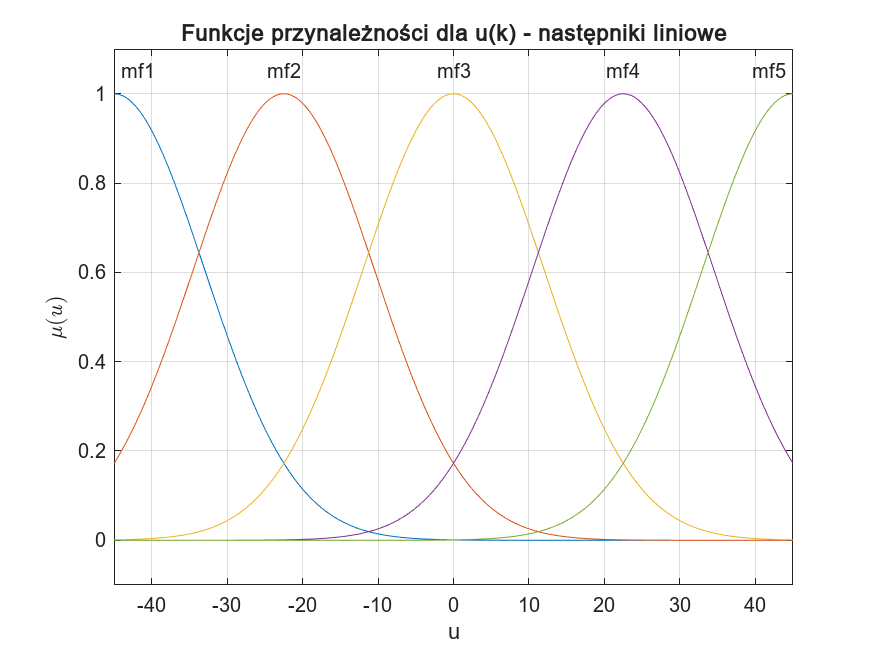
\includegraphics[width=\textwidth]{pictures/hamm_linearFis}
\caption{Zbiory rozmyte - następniki liniowe.}
\end{figure}

Zarówno do budowy modelu, jak i wyznaczenia parametrów następników wykorzystano narzędzia oferowane przez MATLAB w ramach \textit{Fuzzy Logic Toolbox}. Korzystając z funkcji \verb+sugfis()+ zbudowano nieliniowy model rozmyty typu Takagi - Sugeno. Zdecydowano się na pięć zbiorów rozmytych o gaussowskim kształcie, co zapewnia różniczkowalność (SZAU). Następnie, dzięki wykorzystaniu \verb+addInput()+, \verb+addOutput()+, \verb+addMF()+ udało się zbudować bazę reguł - \verb+addRule()+, co bezpośrednio przełożyło się na wyznaczenie współczynników pierwszej iteracji. Konieczne było późniejsze ręczne dostrajanie modelu, które przy względnie dużej liczbie zbiorów nie przysporzyło dużo problemów. Ostatecznie zdefiniowano następujące wartości parametrów następników:

\begin{table}[h!]
\centering
\renewcommand{\arraystretch}{1.2} % Zwiększa wysokość wierszy
\begin{tabular}{|>{\centering\arraybackslash}m{3cm}|>{\centering\arraybackslash}m{3cm}|>{\centering\arraybackslash}m{3cm}|}
\hline
Nr reguły & Współczynnik $a_r$ & Współczynnik $b_r$ \\ \hline
1 & $\num{0.7895}$ & $\num{0.0001}$ \\ \hline
2 & $\num{0.8982}$ & $\num{0.0002}$ \\ \hline
3 & $\num{1.0933}$ & $\num{0.0001}$ \\ \hline
4 & $\num{1.0489}$ & $\num{0}$ \\ \hline
5 & $\num{1.2034}$ & $\num{0.0001}$ \\ \hline
\end{tabular}
\end{table}

\newpage

\subsection{Następniki nieliniowe}
Wprowadzając następniki w postaci hiperbolicznej spodziewano się zachowania dokładności przy jednoczesnym zmniejszeniu liczby zbiorów rozmytych [Robust observer-based controller design for Takagi–Sugeno systems with nonlinear consequent parts]. Sformułowano następującą bazę reguł:

\begin{equation}
\begin{aligned}
\text{Reguła 1: Jeśli} \quad u(k) \quad \text{jest} \quad &U_1, \quad \text{to}: \quad y^1(k) = a_1 \sinh\left(\frac{u(k)}{b_1}\right) \\[10pt]
\text{Reguła 2: Jeśli} \quad u(k) \quad \text{jest} \quad &U_2, \quad \text{to}: \quad y^2(k) = a_2 \sinh\left(\frac{u(k)}{b_2}\right) \\[10pt]
\text{Reguła 3: Jeśli} \quad u(k) \quad \text{jest} \quad &U_3, \quad \text{to}: \quad y^2(k) = a_3 \sinh\left(\frac{u(k)}{b_3}\right)
\end{aligned}
\label{nastepniki_nlin}
\end{equation}

Zgodnie z oczekiwaniami udało się wprowadzić mniejszą liczbę zbiorów rozmytych.

\begin{figure}[h!]
\centering
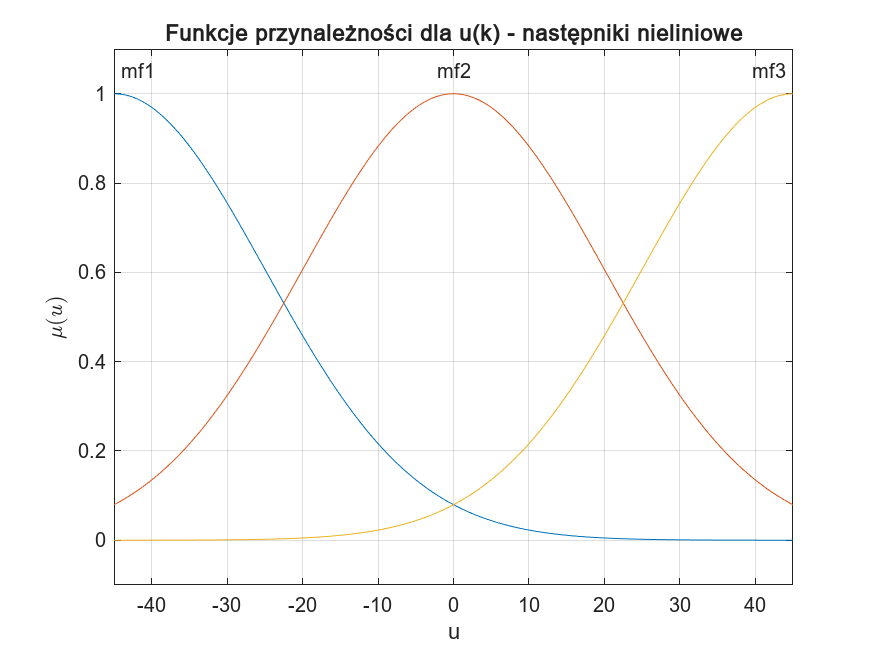
\includegraphics[width=\textwidth]{pictures/hamm_nonlinearFis}
\caption{Zbiory rozmyte - następniki nieliniowe.}
\end{figure}

\newpage

Procedura dostrajania parametrów następników różniła się w stosunku do odpowiedników liniowych. Wynikało to z tego, że wykorzystywane narzędzie do budowy modelu rozmytego domyślnie stroi parametry dla następników liniowych, stąd konieczność znacznej modyfikacji i ręcznego dostrajania. Następnie, po ręcznym dostrojeniu wykorzytsano funkcję z pakietu \textit{Optimization Toolbox}, mianowicie \verb+fminsearch()+. Wybrano taką kolejność ze względu na fakt, że odwracając kolejność, tzn. stosując najpierw metodę Neldera-Meada, otrzymywane wyniki były gorsze niż te wybrane ręcznie. Było to spowodowane skłonnością do wpadania algorytmu w minima lokalne. Istotnym aspektem w tym przypadku okazała się normalizacja argumentu, bowiem kształt funkcji $\sinh()$ zmienia się bardzo gwałtownie dla rosnących wartości zmiennej (rys. {\ref{sinh}}. 

\begin{figure}[h!]
\centering
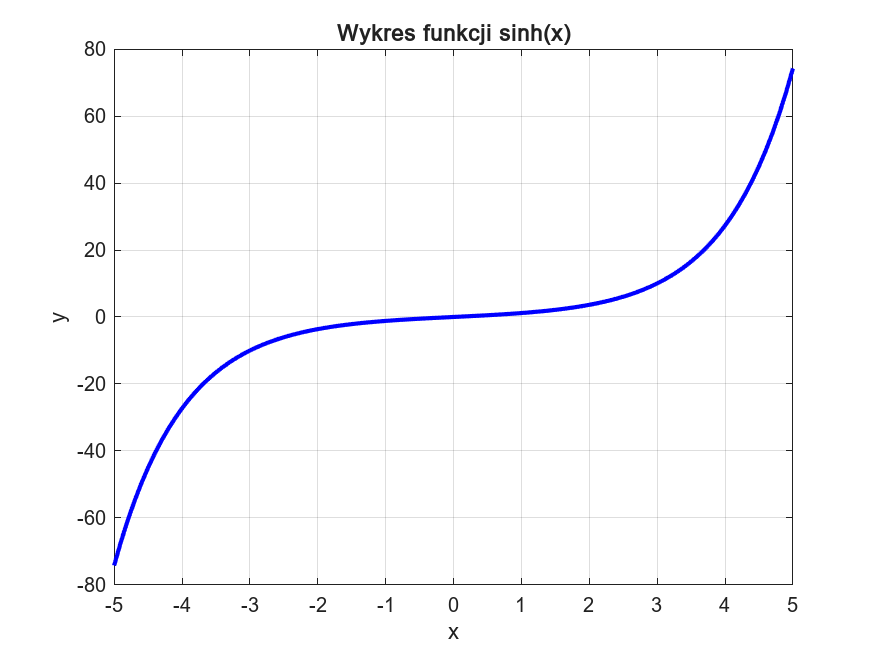
\includegraphics[width=\textwidth]{pictures/sinh}
\caption{Wykres funkcji $\sinh()$.}
\label{sinh}
\end{figure}

Ostateczne wartości współczynników następników reguł zebrano w tab. \ref{nonlinear_coeff}.

\begin{table}[h!]
\centering
\renewcommand{\arraystretch}{1.2} % Zwiększa wysokość wierszy
\begin{tabular}{|>{\centering\arraybackslash}m{2cm}|>{\centering\arraybackslash}m{3cm}|>{\centering\arraybackslash}m{3cm}|}
\hline
Nr reguły & Współczynnik $a_r$ & Współczynnik $b_r$ \\ \hline
1. & $\num{46.4941}$ & $\num{62.8862}$ \\ \hline
2. & $\num{36.2347}$ & $\num{36.2592}$ \\ \hline
3. & $\num{110.4841}$ & $\num{98.7690}$ \\ \hline    
\end{tabular}
\caption{Współczynniki hiperbolicznych następników reguł.}
\label{nonlinear_coeff}
\end{table}

\newpage

\subsection{Porównanie}
Dostroiwszy oba modele przyszedł czas na ich porównanie. Wygenerowano pięć sekwencji losowo zmieniającego się sygnału sterującego, następnie wynik został porównany do rezultatu uzyskanego dla modelu nieliniowego - wzorcowego - obliczonego za pomocą zmodyfikowanej metody Eulera. Wskaźnikiem porównawczym był błąd średnio kwadratowy. Aby zaznaczyć jakie korzyści wnosi nieliniowa część modelu Hammersteina na dokładność modelowania, w każdej sekwencji obliczono także wskaźnik dla modelu liniowego.

\begin{figure}[h!]
\centering
\subfloat[Następniki liniowe]{
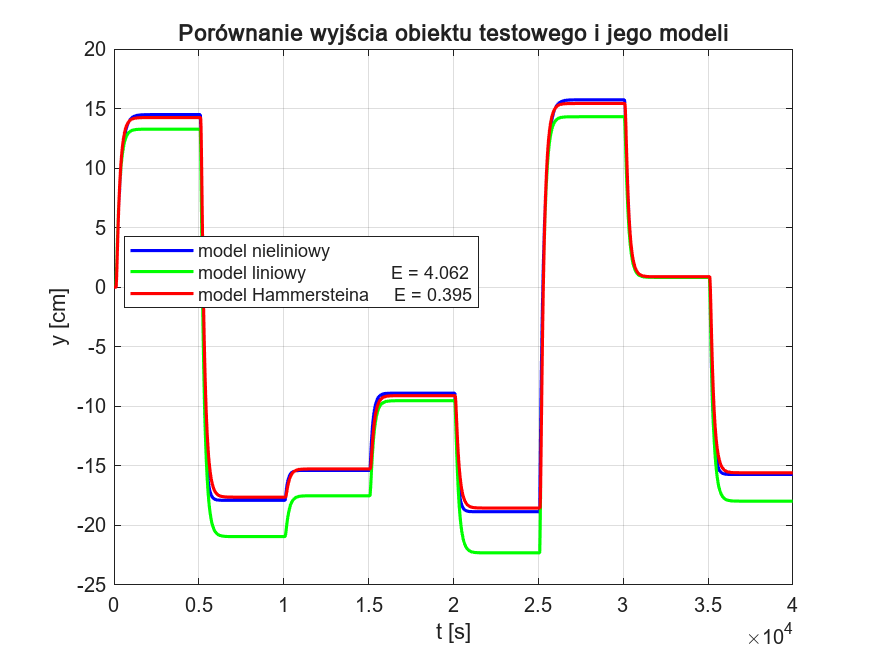
\includegraphics[width=0.7\textwidth]{pictures/HammersteinLinearModel_1}}
\vspace{0.5cm}
\subfloat[Następniki nieliniowe]{
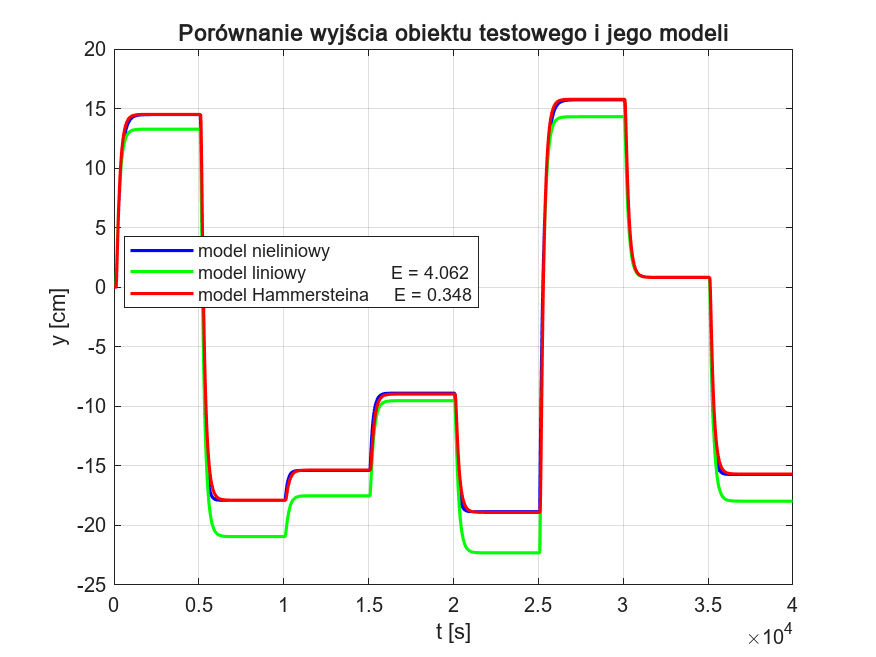
\includegraphics[width=0.7\textwidth]{pictures/HammersteinNonlinearModel_1}}
\caption{Porównanie modelu Hammersteina z następnikami liniowymi i nieliniowymi - pierwsza sekwencja.}
\label{first_hamm}
\end{figure}

\begin{figure}[p]
\centering
\subfloat[Następniki liniowe]{
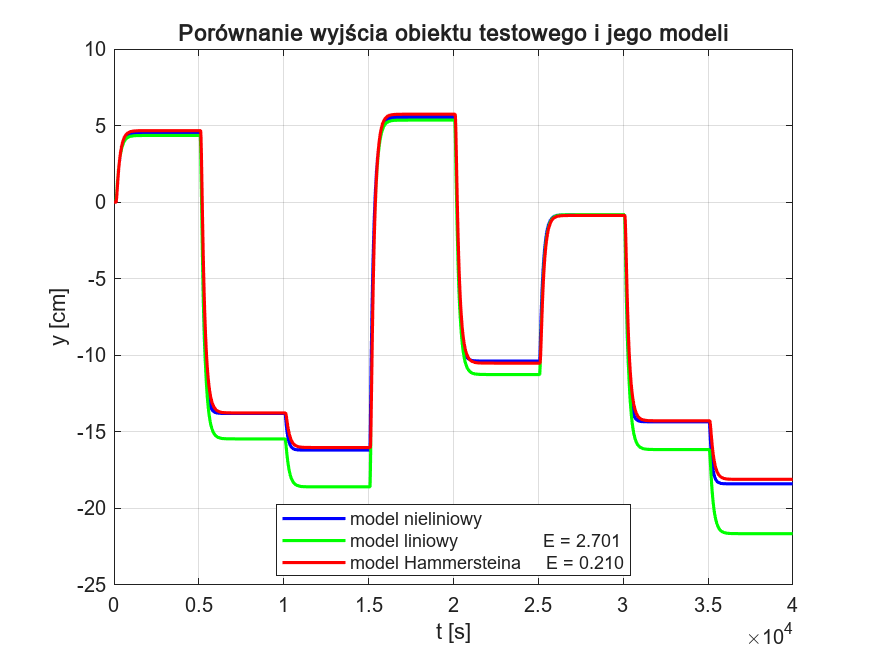
\includegraphics[width=0.75\textwidth]{pictures/HammersteinLinearModel_2}}
\vspace{0.5cm}
\subfloat[Następniki nieliniowe]{
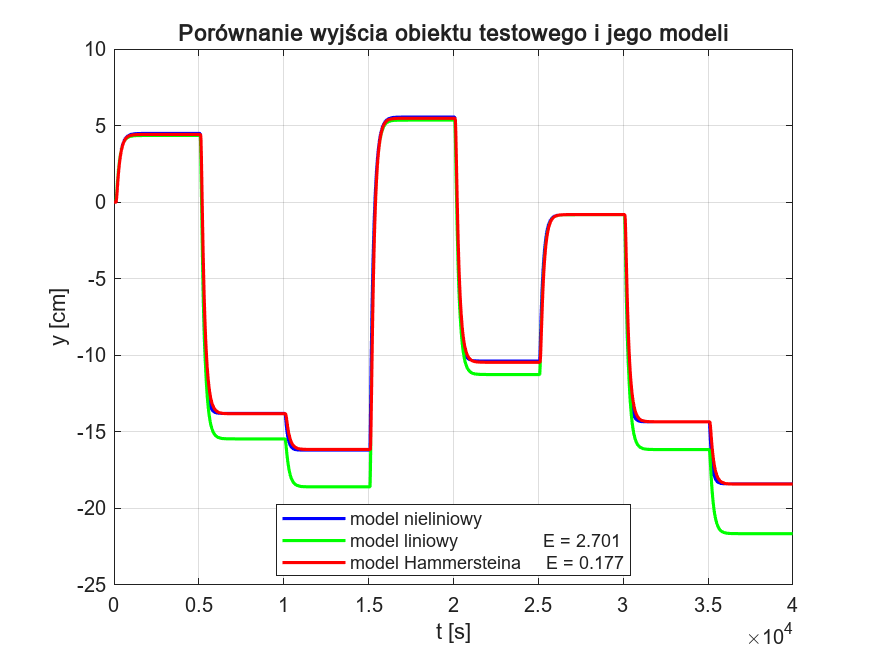
\includegraphics[width=0.75\textwidth]{pictures/HammersteinNonlinearModel_2}}
\caption{Porównanie modelu Hammersteina z następnikami liniowymi i nieliniowymi - druga sekwencja.}
\end{figure}

\begin{figure}[p]
\centering
\subfloat[Następniki liniowe]{
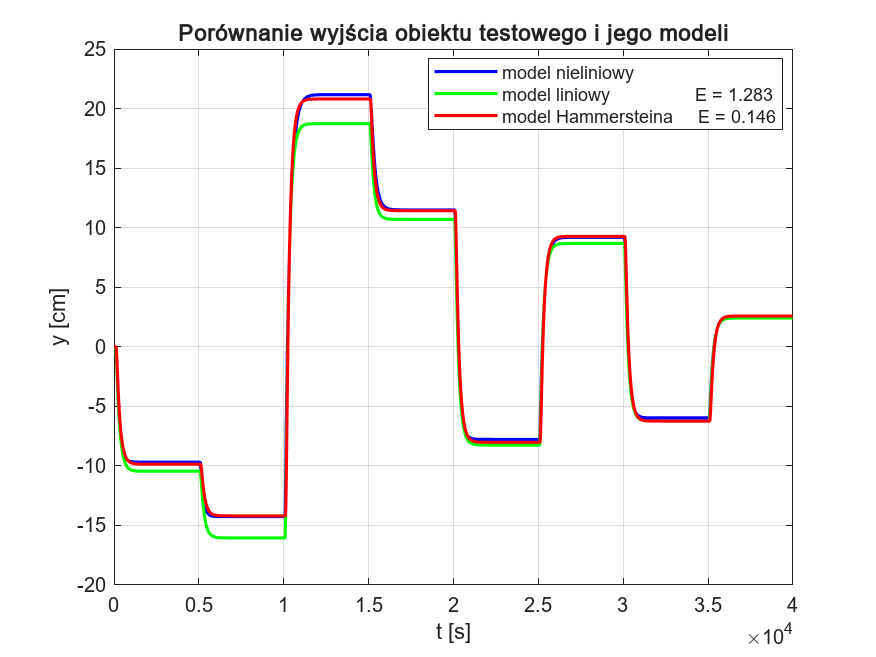
\includegraphics[width=0.75\textwidth]{pictures/HammersteinLinearModel_3}}
\vspace{0.5cm}
\subfloat[Następniki nieliniowe]{
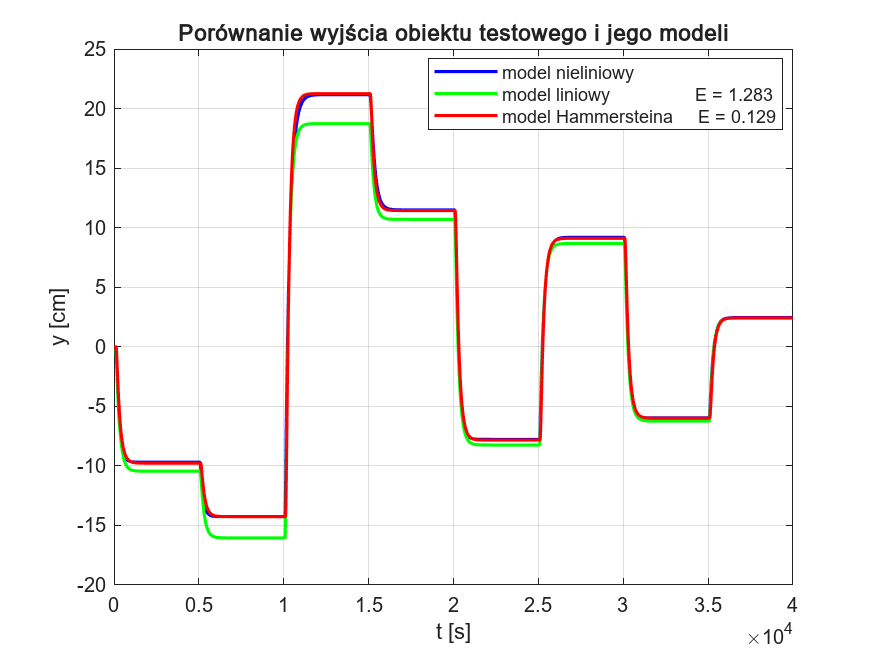
\includegraphics[width=0.75\textwidth]{pictures/HammersteinNonlinearModel_3}}
\caption{Porównanie modelu Hammersteina z następnikami liniowymi i nieliniowymi - trzecia sekwencja.}
\end{figure}

\begin{figure}[p]
\centering
\subfloat[Następniki liniowe]{
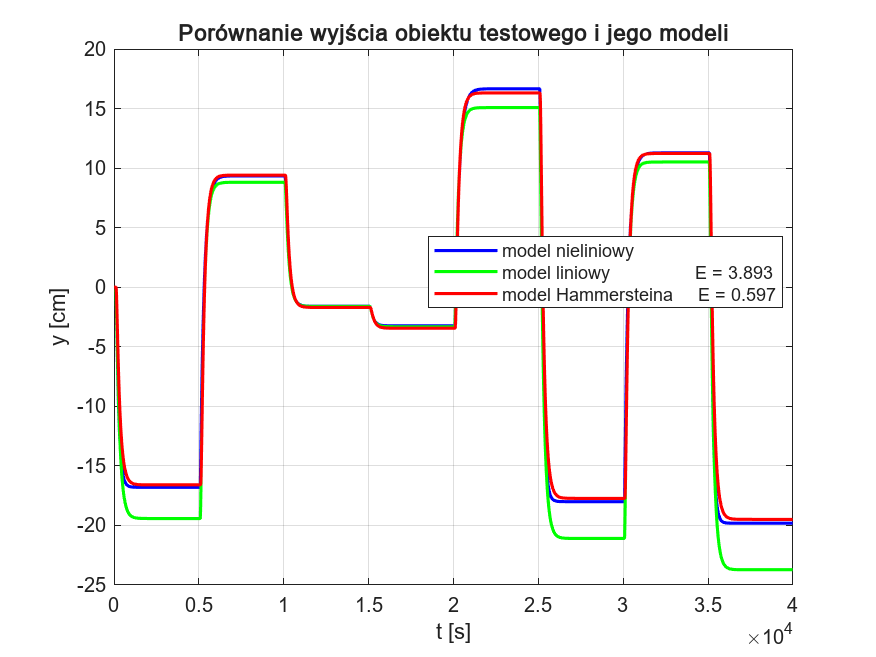
\includegraphics[width=0.75\textwidth]{pictures/HammersteinLinearModel_4}}
\vspace{0.5cm}
\subfloat[Następniki nieliniowe]{
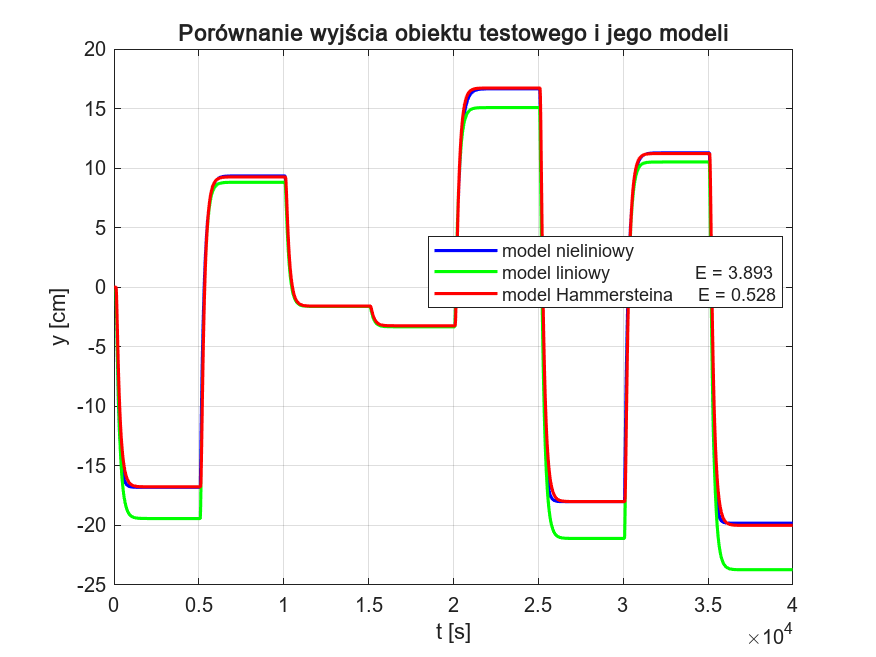
\includegraphics[width=0.75\textwidth]{pictures/HammersteinNonlinearModel_4}}
\caption{Porównanie modelu Hammersteina z następnikami liniowymi i nieliniowymi - czwarta sekwencja.}
\end{figure}

\begin{figure}[p]
\centering
\subfloat[Następniki liniowe]{
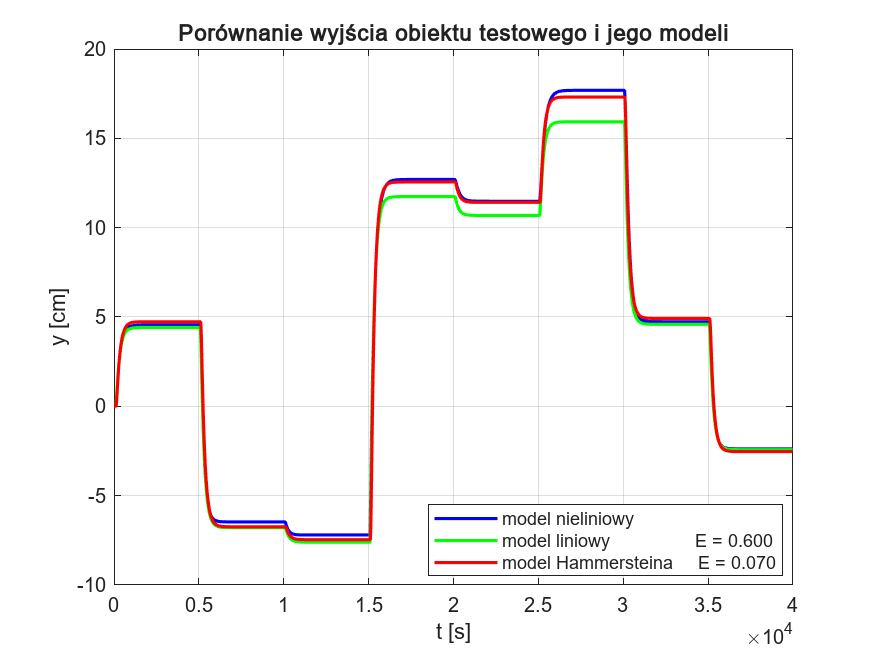
\includegraphics[width=0.75\textwidth]{pictures/HammersteinLinearModel_5}}
\vspace{0.5cm}
\subfloat[Następniki nieliniowe]{
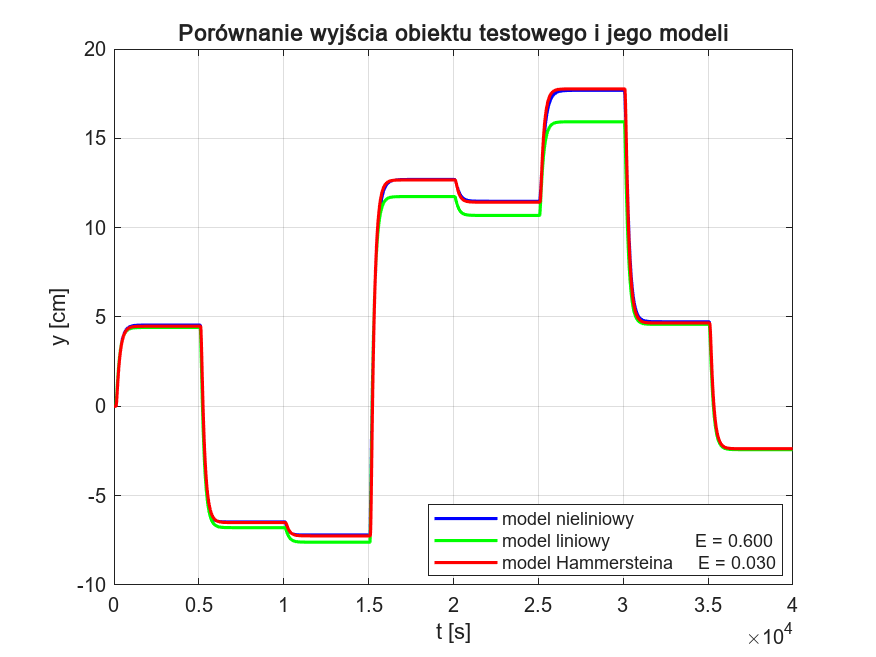
\includegraphics[width=0.75\textwidth]{pictures/HammersteinNonlinearModel_5}}
\caption{Porównanie modelu Hammersteina z następnikami liniowymi i nieliniowymi - piąta sekwencja.}
\label{last_hamm}
\end{figure}

\newpage

Zaprezentowane wykresy na rys. \ref{first_hamm} - \ref{last_hamm} ilustrują przede wszystkim zysk zastosowania modelu Hammersteina do opisu obiektu. Otrzymane wyniki są nieporównywalnie lepsze w stosunku do modelu liniowego. Natomiast przyglądając się z bliska, można zauważyć również poprawę dzięki wprowadzeniu dodatkowej nieliniowości w definicji następników rozmytego modelu typu Takagi-Sugeno. W tab. \ref{comparison_hamm} zebrano uzyskane wyniki.

\begin{table}[h!]
\centering
\renewcommand{\arraystretch}{1.2}
\begin{tabular}{|>{\centering\arraybackslash}m{2cm}|>{\centering\arraybackslash}m{3cm}|>{\centering\arraybackslash}m{3cm}|>{\centering\arraybackslash}m{3cm}|}
\hline
\multirow{2}{*}{Nr sekwencji} & \multirow{2}{*}{Model liniowy} & \multicolumn{2}{c|}{Model Hammersteina} \\ \cline{3-4}
 &  & Następniki liniowe & Następniki nieliniowe \\ \hline
1. & $\num{4.062}$ & $\num{0.395}$ & $\num{0.348}$ \\ \hline
2. & $\num{2.701}$ & $\num{0.210}$ & $\num{0.177}$ \\ \hline
3. & $\num{1.283}$ & $\num{0.146}$ & $\num{0.129}$ \\ \hline
4. & $\num{3.893}$ & $\num{0.597}$ & $\num{0.528}$ \\ \hline
5. & $\num{0.600}$ & $\num{0.070}$ & $\num{0.030}$ \\ \hline
\end{tabular}
\caption{Porównanie modeli.}
\label{comparison_hamm}
\end{table}

Należy pamiętać, że w przypadku następników hiperbolicznych zredukowano liczbę zbiorów rozmytych. Zatem udało się poprawić dokładność modelowania, przy jednoczesnym zmniejszeniu liczby reguł modelu TS.
\section{Model Wienera}
Model Wienera to struktura nieliniowego systemu, w której liniowy blok dynamiczny jest umieszczony przed nieliniowym blokiem statycznym. Oznacza to, że najpierw wejście przechodzi przez liniowy filtr, a następnie poddawane jest nieliniowej transformacji. Modele Wienera są szczególnie użyteczne w systemach, gdzie obserwowana nieliniowość wynika głównie z ograniczeń lub nasycenia elementów wykonawczych, takich jak silniki, zawory, czy inne elementy mechaniczne.  Zatem istota tego modeli jest taka sama jak w przypadku modelu Hammersteina - oddzielenie nieliniowej statyki od liniowej dynamiki - z tym, że nieliniową statykę poprzedzono liniową dynamika - odwrotnie niż jak to było w przypadku omówionego modelu, co graficznie zilustrowano na rys. \ref{wien_model}.

\begin{figure}[h!]
\centering
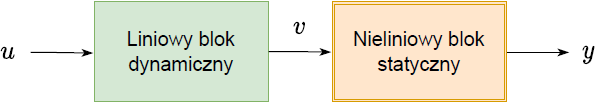
\includegraphics[width=\textwidth]{pictures/wien_model}
\caption{Reprezentacja graficzna modelu Wienera.}
\label{wien_model}
\end{figure}

Sygnał wejściowy trafia na liniowy blok dynamiczny, którego wyjściem jest przekonwertowany sygnał $v = f(u)$, który następnie trafia na nieliniową statykę, której wyjściem jest sygnał $y$.

Warto podkreślić, że modele Wienera jest trudniejszy w interpretacji niż model Hammersteina. Wynika to z tego, że sygnał wejściowy przechodzi najpierw przez system liniowy, a dopiero potem przez nieliniowy element, co utrudnia analizę wpływu nieliniowości. Dodatkowo, sygnał po filtracji liniowej może mieć bardziej złożone właściwości, co komplikuje ocenę jego zachowania w bloku nieliniowym, a także może przełożyć się na bardziej wymagającą estymacja parametrów w modelu.

\subsection{Następniki}
Zarówno w przypadku następników liniowych, jak i hiperbolicznych wykorzystano dokładnie te same definicje, jakie zastosowano w przypadku modelu Hammersteina - opisane wzorami \ref{nastepniki_lin} oraz \ref{nastepniki_nlin}. Przypomniano jedynie ogólną strukturę poszczególnych reguł.

\begin{description}
\item Następniki liniowe:
\begin{equation}
\text{Reguła n: Jeśli} \quad u(k) \quad \text{jest} \quad U_n, \quad \text{to}: \quad y^n(k) = a_n u(k) + b_n \\[10pt]
\end{equation}

\item Następniki hiperboliczne:
\begin{equation}
\text{Reguła n: Jeśli} \quad u(k) \quad \text{jest} \quad U_n, \quad \text{to}: \quad y^n(k) = a_n \sinh\left(\frac{u(k)}{b_n}\right) \\[10pt]
\end{equation}
\end{description}

\newpage

Nie uległa zmianie również liczba i postać zbiorów rozmytych - zmienił się jedynie zakres rozmywania. 

\begin{figure}[h!]
\centering
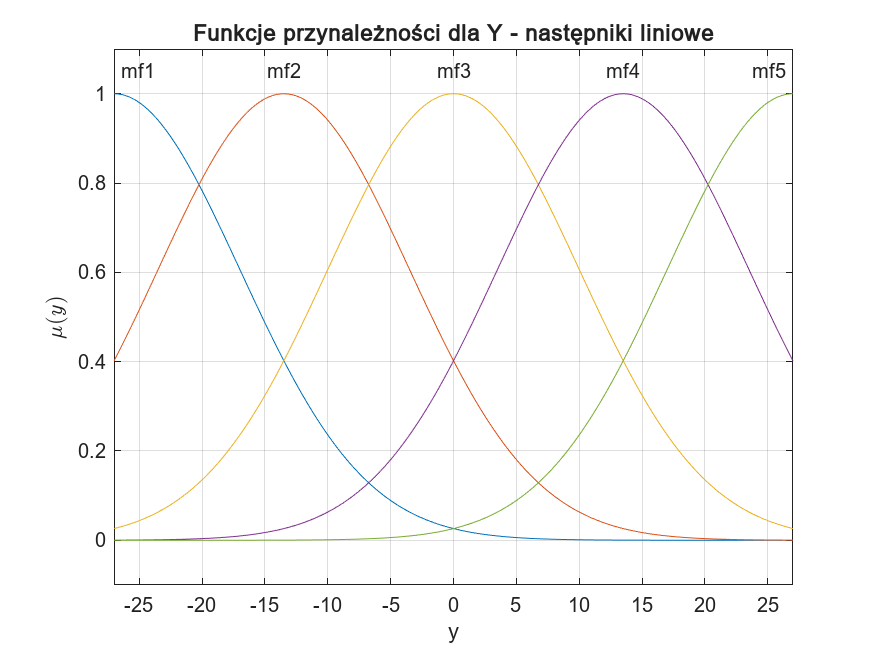
\includegraphics[width=0.85\textwidth]{pictures/WienerfuzzySets_liniowe}
\caption{Zbiory rozmyte - następniki liniowe.}
\end{figure}

\vfill

\begin{figure}[h!]
\centering
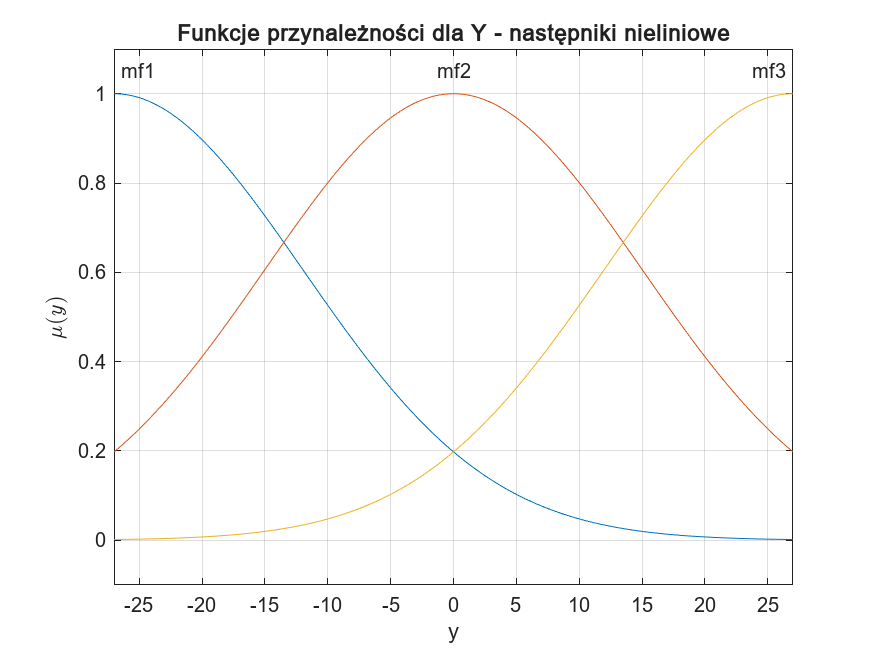
\includegraphics[width=0.85\textwidth]{pictures/WienerfuzzySets_nieliniowe}
\caption{Zbiory rozmyte - następniki nieliniowe.}
\end{figure}

\newpage

\subsection{Porównanie}

Procedura porównawcza wyglądała identycznie jak w przypadku modelu Hammersteina, tj. dla tych samych wygenerowanych sekwencji sygnału sterującego wyznaczono odpowiedzi modelu nieliniowego, liniowego, modelu Wienera z następnikami liniowymi oraz hiperbolicznymi. Przebiegi przedstawiono na rys. \ref{first_wien} - \ref{last_wien}, natomiast dane liczbowe zgromadzono w tab. \ref{comparison_wien}.

\begin{figure}[h!]
\centering
\subfloat[Następniki liniowe]{
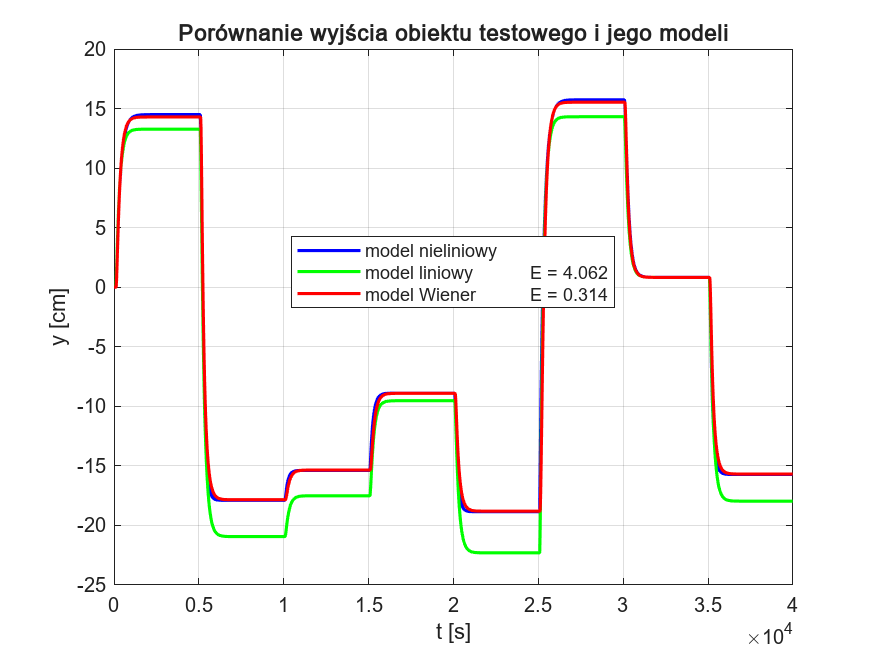
\includegraphics[width=0.7\textwidth]{pictures/WienerLinearModel_1}}
\vspace{0.5cm}
\subfloat[Następniki nieliniowe]{
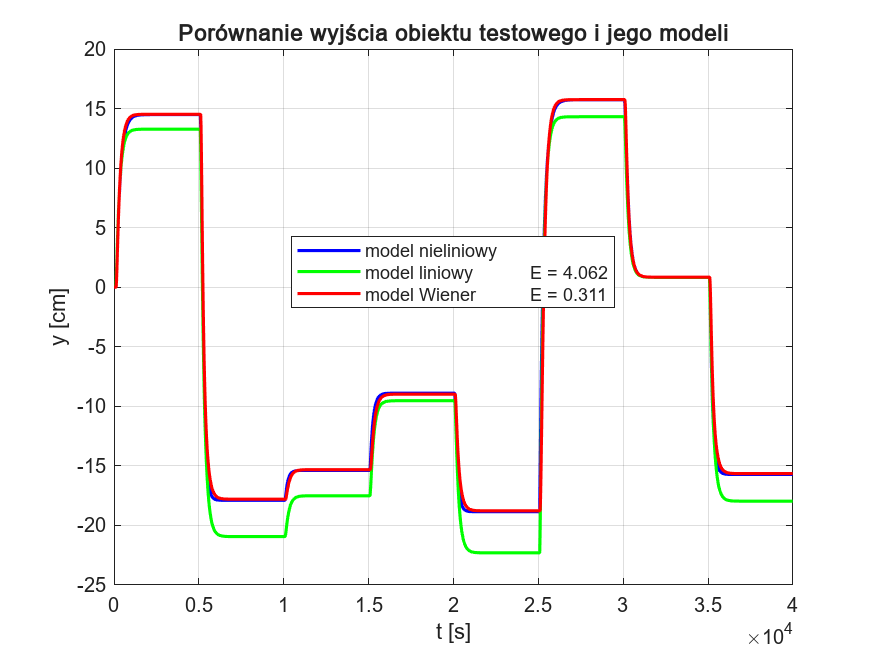
\includegraphics[width=0.7\textwidth]{pictures/WienerNonlinearModel_1}}
\caption{Porównanie modelu Wienera z następnikami liniowymi i nieliniowymi - pierwsza sekwencja.}
\label{first_wien}
\end{figure}

\begin{figure}[p]
\centering
\subfloat[Następniki liniowe]{
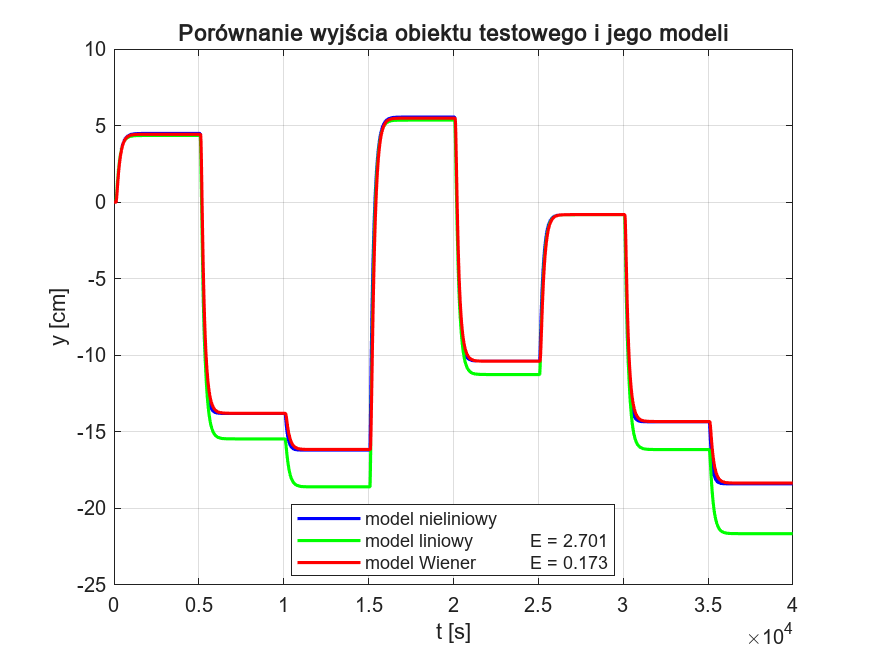
\includegraphics[width=0.75\textwidth]{pictures/WienerLinearModel_2}}
\vspace{0.5cm}
\subfloat[Następniki nieliniowe]{
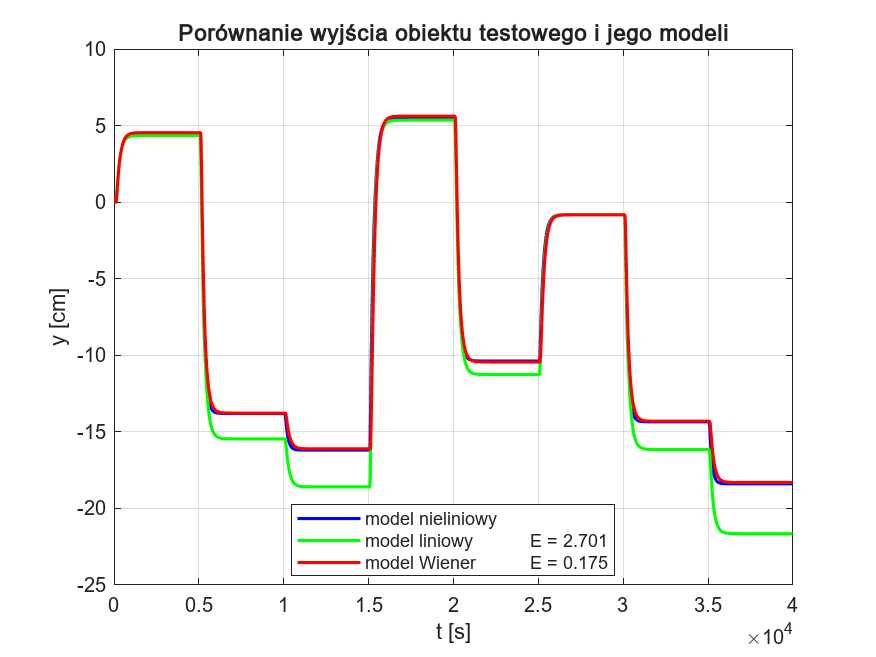
\includegraphics[width=0.75\textwidth]{pictures/WienerNonlinearModel_2}}
\caption{Porównanie modelu Wienera z następnikami liniowymi i nieliniowymi - druga sekwencja.}
\end{figure}

\begin{figure}[p]
\centering
\subfloat[Następniki liniowe]{
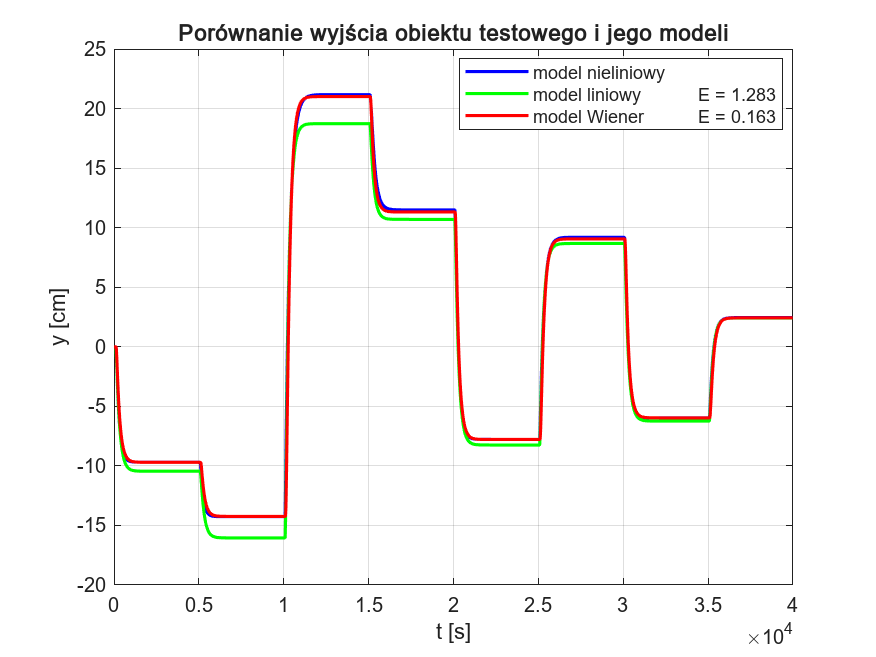
\includegraphics[width=0.75\textwidth]{pictures/WienerLinearModel_3}}
\vspace{0.5cm}
\subfloat[Następniki nieliniowe]{
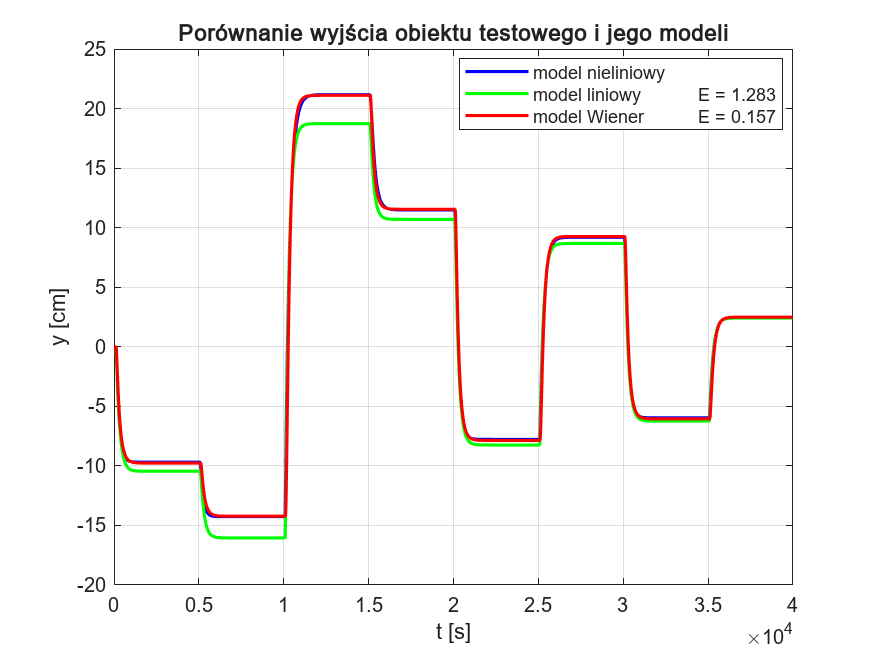
\includegraphics[width=0.75\textwidth]{pictures/WienerNonlinearModel_3}}
\caption{Porównanie modelu Wienera z następnikami liniowymi i nieliniowymi - trzecia sekwencja.}
\end{figure}

\begin{figure}[p]
\centering
\subfloat[Następniki liniowe]{
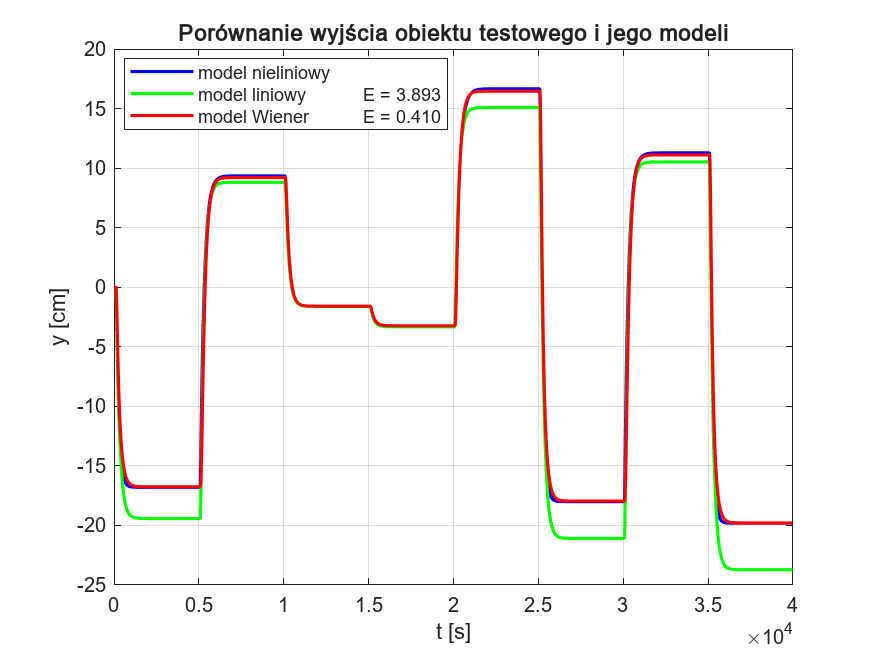
\includegraphics[width=0.75\textwidth]{pictures/WienerLinearModel_4}}
\vspace{0.5cm}
\subfloat[Następniki nieliniowe]{
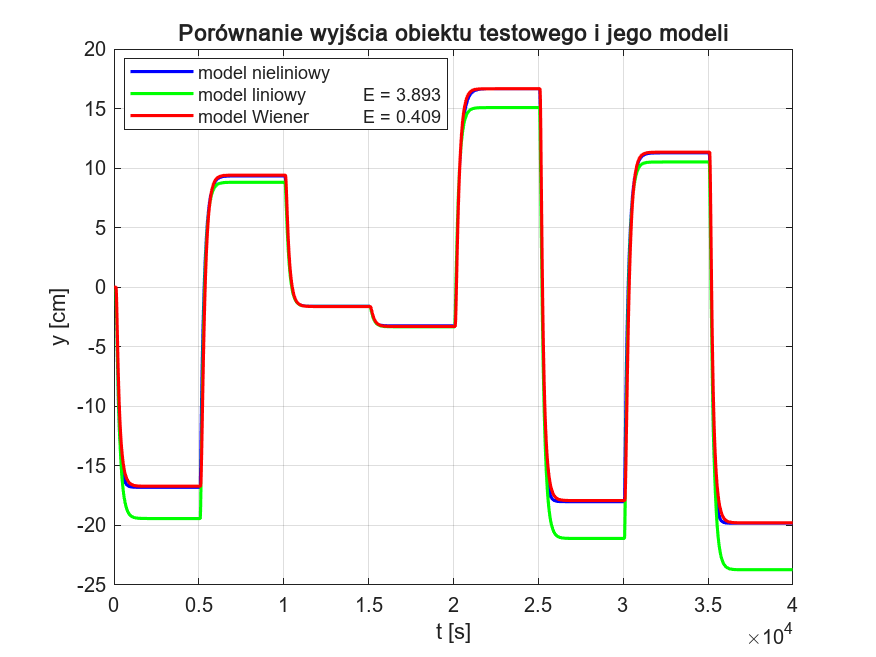
\includegraphics[width=0.75\textwidth]{pictures/WienerNonlinearModel_4}}
\caption{Porównanie modelu Wienera z następnikami liniowymi i nieliniowymi - czwarta sekwencja.}
\end{figure}

\begin{figure}[p]
\centering
\subfloat[Następniki liniowe]{
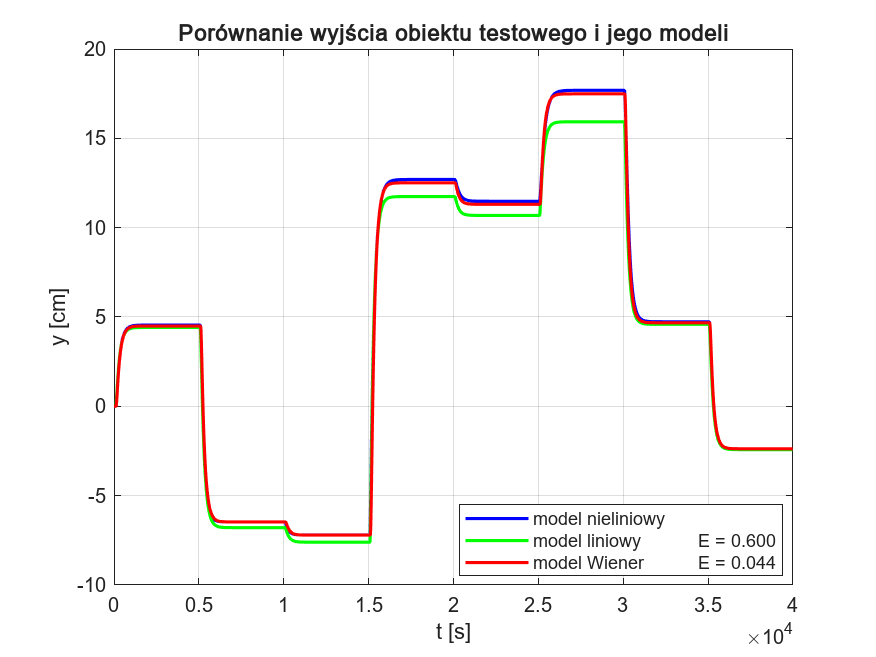
\includegraphics[width=0.75\textwidth]{pictures/WienerLinearModel_5}}
\vspace{0.5cm}
\subfloat[Następniki nieliniowe]{
\includegraphics[width=0.75\textwidth]{pictures/WienerNonlinearModel_5}}
\caption{Porównanie modelu Wienera z następnikami liniowymi i nieliniowymi - piąta sekw encja.}
\label{last_wien}
\end{figure}

\newpage

Wyniki zebrane w tab. \ref{comparison_wien} dla modelu Wienera z następnikami liniowymi i nieliniowymi są niemalże identyczne, a ewentualne różnice są pomijalne. Porównując otrzymane rezultaty z tymi otrzymanymi w przypadku modelu Hammersteina okazuje się, że model Wienera jest nieco lepszy, co może wskazywać na większe nieliniowości na wyjściu procesu.
 
\begin{table}[h!]
\centering
\renewcommand{\arraystretch}{1.2}
\begin{tabular}{|>{\centering\arraybackslash}m{2cm}|>{\centering\arraybackslash}m{3cm}|>{\centering\arraybackslash}m{3cm}|>{\centering\arraybackslash}m{3cm}|}
\hline
\multirow{2}{*}{Nr sekwencji} & \multirow{2}{*}{Model liniowy} & \multicolumn{2}{c|}{Model Wienera} \\ \cline{3-4}
 &  & Następniki liniowe & Następniki nieliniowe \\ \hline
1. & $\num{4.062}$ & $\num{0.314}$ & $\num{0.311}$ \\ \hline
2. & $\num{2.701}$ & $\num{0.173}$ & $\num{0.175}$ \\ \hline
3. & $\num{1.283}$ & $\num{0.163}$ & $\num{0.157}$ \\ \hline
4. & $\num{3.893}$ & $\num{0.410}$ & $\num{0.409}$ \\ \hline
5. & $\num{0.600}$ & $\num{0.044}$ & $\num{0.035}$ \\ \hline
\end{tabular}
\caption{Porównanie modeli.}
\label{comparison_wien}
\end{table}

Udało się osiągnąć zamierzony efekt - mniejsza liczba reguł, bez utraty dokładności.

\section{Regulacja predykcyjna}
Współczesne systemy sterowania wymagają metod, które potrafią skutecznie przewidywać i reagować na zmieniające się warunki pracy obiektów. Regulacja predykcyjna stanowi jedno z najbardziej zaawansowanych podejść do sterowania, pozwalając na optymalne korygowanie trajektorii sterowania w czasie rzeczywistym. Dzięki wykorzystaniu modeli matematycznych układu oraz przewidywaniu jego przyszłych stanów, MPC, a w szczególności DMC, umożliwia uwzględnienie ograniczeń oraz minimalizację błędów sterowania.

W kontekście systemów nieliniowych szczególnie przydatne okazują się modele Hammersteina i Wienera, które rozdzielając nieliniową statykę od liniowej dynamiki układu ułatwiają implementację algorytmów predykcyjnych, ponieważ liniowa część modelu może być efektywnie analizowana i przewidywana przy użyciu klasycznych technik optymalizacyjnych, podczas gdy nieliniowa statyka może być traktowana jako dodatkowa warstwa przekształcająca sygnały sterowania lub wyjścia. Dzięki temu możliwe jest skuteczne sterowanie szeroką gamą obiektów przemysłowych, od procesów chemicznych po nowoczesne systemy robotyczne i autonomiczne. W niniejszym rozdziale zostaną omówione kluczowe zasady działania regulacji predykcyjnej oraz sposoby jej zastosowania w połączeniu z modelami Hammersteina i Wienera.

\subsection{Regulator DMC}
Tu coś o DMC, może jakiś schemacik blokowy

\newpage

 
\subsection{Porównanie}

\begin{table}[h!]
\centering
\renewcommand{\arraystretch}{1.2}
\begin{tabular}{|>{\centering\arraybackslash}m{2.5cm}|>{\centering\arraybackslash}m{2.5cm}|>{\centering\arraybackslash}m{2.5cm}|>{\centering\arraybackslash}m{2.5cm}|>{\centering\arraybackslash}m{2.5cm}|}
\hline
\multirow{2}{*}{Regulator} & \multicolumn{2}{c|}{Model Hammersteina} & \multicolumn{2}{c|}{Model Wienera} \\ \cline{2-5}
 & Następniki liniowe & Następniki nieliniowe & Następniki liniowe & Następniki nieliniowe \\ \hline
DMC-analitic & $\num{20.6110}$ & $\num{20.4929}$ & $\num{22.3904}$ & $\num{22.4372}$ \\ \hline
DMC-numeric & $\num{20.6110}$ & $\num{20.4929}$ & $\num{22.3903}$ & $\num{22.4372}$ \\ \hline
DMC-SL & $\num{20.5775}$ & $\num{20.4629}$ & $\num{22.3721}$ & $\num{22.4176}$ \\ \hline
DMC-NPL & $\num{20.4963}$ & $\num{20.3846}$ & $\num{22.3008}$ & $\num{22.3467}$ \\ \hline
FDMC & $\num{19.7474}$ & $\num{19.6734}$ & $\num{21.6466}$ & $\num{21.7162}$ \\ \hline
\end{tabular}
\caption{Porównanie modeli.}
\end{table}

\begin{table}[h!]
\centering
\renewcommand{\arraystretch}{1.2}
\begin{tabular}{|>{\centering\arraybackslash}m{2.5cm}|>{\centering\arraybackslash}m{1.25cm}|>{\centering\arraybackslash}m{1.25cm}|>{\centering\arraybackslash}m{1.25cm}|>{\centering\arraybackslash}m{1.25cm}|>{\centering\arraybackslash}m{1.25cm}|>{\centering\arraybackslash}m{1.25cm}|>{\centering\arraybackslash}m{1.25cm}|
>{\centering\arraybackslash}m{1.25cm}|}
\hline
\multirow{3}{*}{Regulator} & \multicolumn{4}{c|}{Model Hammersteina} & \multicolumn{4}{c|}{Model Wienera} \\ \cline{2-9}
 & \multicolumn{2}{c|}{\parbox{2.5cm}{\centering Następniki liniowe}} & \multicolumn{2}{c|}{\parbox{2.5cm}{\centering Następniki nieliniowe}} & \multicolumn{2}{c|}{\parbox{2.5cm}{\centering Następniki liniowe}} & \multicolumn{2}{c|}{\parbox{2.5cm}{\centering Następniki nieliniowe}} \\ \cline{2-9}
 & $\text{E}_\text{y}$ & $\text{E}_\text{u}$ & $\text{E}_\text{y}$ & $\text{E}_\text{u}$ & $\text{E}_\text{y}$ & $\text{E}_\text{u}$ & $\text{E}_\text{y}$ & $\text{E}_\text{u}$ \\ \hline
DMC-analitic & $\num{19.6366}$ & $\num{0.9743}$ & $\num{19.4785}$ & $\num{1.0144}$ & $\num{21.3817}$ & $\num{1.0087}$ & $\num{21.428}$ & $\num{1.0092}$ \\ \hline
DMC-numeric & $\num{19.6366}$ & $\num{0.9743}$ & $\num{19.4785}$ & $\num{1.0144}$ & $\num{21.3817}$ & $\num{1.0087}$ & $\num{21.428}$ & $\num{1.0092}$ \\ \hline
DMC-SL& $\num{19.5959}$ & $\num{0.9816}$ & $\num{19.4414}$ & $\num{1.0215}$ & $\num{21.3607}$ & $\num{1.0114}$ & $\num{21.4057}$ & $\num{1.0119}$ \\ \hline
DMC-NPL & $\num{19.527}$ & $\num{0.9693}$ & $\num{19.3757}$ & $\num{1.0089}$ & $\num{21.3023}$ & $\num{0.99852}$ & $\num{21.3476}$ & $\num{0.99906}$ \\ \hline
FDMC& $\num{18.2132}$ & $\num{1.5342}$ & $\num{18.1112}$ & $\num{1.5622}$ & $\num{20.0199}$ & $\num{1.6267}$ & $\num{20.0874}$ & $\num{1.6288}$ \\ \hline
\end{tabular}
\caption{Porównanie modeli.}
\end{table}

%%%%%%%%%%%%%%%%%%%%% ANALITIC %%%%%%%%%%%%%%%%%%%%%

\newgeometry{left=1cm, right=1cm, top=2cm, bottom=2cm}
\begin{figure}[p]
\centering
\begin{minipage}{0.495\linewidth}
    \centering
    \includegraphics[width=1.1\linewidth]{pictures/DMC_analitic_y}
\end{minipage}
\hfill
\begin{minipage}{0.495\linewidth}
    \centering
    \includegraphics[width=1.1\linewidth]{pictures/DMC_analitic_u}
\end{minipage}

\caption{Porównanie sygnału wyjściowego oraz sterującego poszczególnych modeli.}

\vspace{2cm}

\begin{minipage}{0.495\linewidth}
    \centering
    \includegraphics[width=\linewidth]{pictures/DMC_analitic_y_zoom}
\end{minipage}
\hfill
\begin{minipage}{0.495\linewidth}
    \centering
    \includegraphics[width=\linewidth]{pictures/DMC_analitic_u_zoom}
\end{minipage}
\caption{Wyszczególnienie interesujących fragmentów przebiegów.}
\end{figure}

%%%%%%%%%%%%%%%%%%%%% NUMERIC %%%%%%%%%%%%%%%%%%%%%

\begin{figure}[p]
\centering
\begin{minipage}{0.495\linewidth}
    \centering
    \includegraphics[width=1.1\linewidth]{pictures/DMC_numeric_y}
\end{minipage}
\hfill
\begin{minipage}{0.495\linewidth}
    \centering
    \includegraphics[width=1.1\linewidth]{pictures/DMC_numeric_u}
\end{minipage}

\caption{Porównanie sygnału wyjściowego oraz sterującego poszczególnych modeli.}

\vspace{2cm} 

\begin{minipage}{0.495\linewidth}
    \centering
    \includegraphics[width=\linewidth]{pictures/DMC_numeric_y_zoom}
\end{minipage}
\hfill
\begin{minipage}{0.495\linewidth}
    \centering
    \includegraphics[width=\linewidth]{pictures/DMC_numeric_u_zoom}
\end{minipage}
\caption{Wyszczególnienie interesujących fragmentów przebiegów.}
\end{figure}

%%%%%%%%%%%%%%%%%%%%% SL %%%%%%%%%%%%%%%%%%%%%

\begin{figure}[p]
\centering
\begin{minipage}{0.495\linewidth}
    \centering
    \includegraphics[width=1.1\linewidth]{pictures/DMC_sl_y}
\end{minipage}
\hfill
\begin{minipage}{0.495\linewidth}
    \centering
    \includegraphics[width=1.1\linewidth]{pictures/DMC_sl_u}
\end{minipage}

\caption{Porównanie sygnału wyjściowego oraz sterującego poszczególnych modeli.}

\vspace{2cm} 

\begin{minipage}{0.495\linewidth}
    \centering
    \includegraphics[width=\linewidth]{pictures/DMC_sl_y_zoom}
\end{minipage}
\hfill
\begin{minipage}{0.495\linewidth}
    \centering
    \includegraphics[width=\linewidth]{pictures/DMC_sl_u_zoom}
\end{minipage}
\caption{Wyszczególnienie interesujących fragmentów przebiegów.}
\end{figure}

%%%%%%%%%%%%%%%%%%%%% NPL %%%%%%%%%%%%%%%%%%%%%

\begin{figure}[p]
\centering
\begin{minipage}{0.495\linewidth}
    \centering
    \includegraphics[width=1.1\linewidth]{pictures/DMC_npl_y}
\end{minipage}
\hfill
\begin{minipage}{0.495\linewidth}
    \centering
    \includegraphics[width=1.1\linewidth]{pictures/DMC_npl_u}
\end{minipage}

\caption{Porównanie sygnału wyjściowego oraz sterującego poszczególnych modeli.}

\vspace{2cm} 

\begin{minipage}{0.495\linewidth}
    \centering
    \includegraphics[width=\linewidth]{pictures/DMC_npl_y_zoom}
\end{minipage}
\hfill
\begin{minipage}{0.495\linewidth}
    \centering
    \includegraphics[width=\linewidth]{pictures/DMC_npl_u_zoom}
\end{minipage}
\caption{Wyszczególnienie interesujących fragmentów przebiegów.}
\end{figure}

%%%%%%%%%%%%%%%%%%%%% FUZZY %%%%%%%%%%%%%%%%%%%%%

\begin{figure}[p]
\centering
\begin{minipage}{0.495\linewidth}
    \centering
    \includegraphics[width=1.1\linewidth]{pictures/DMC_fuzzy_y}
\end{minipage}
\hfill
\begin{minipage}{0.495\linewidth}
    \centering
    \includegraphics[width=1.1\linewidth]{pictures/DMC_fuzzy_u}
\end{minipage}

\caption{Porównanie sygnału wyjściowego oraz sterującego poszczególnych modeli.}

\vspace{2cm} 

\begin{minipage}{0.495\linewidth}
    \centering
    \includegraphics[width=\linewidth]{pictures/DMC_fuzzy_y_zoom}
\end{minipage}
\hfill
\begin{minipage}{0.495\linewidth}
    \centering
    \includegraphics[width=\linewidth]{pictures/DMC_fuzzy_u_zoom}
\end{minipage}
\caption{Wyszczególnienie interesujących fragmentów przebiegów.}
\end{figure}
\restoregeometry

\newpage

\section{Podsumowanie}







%\chapter{Obiekt badawczy}
%\section{Model Hammersteina}
%\section{Model Wienera}
%\section{Regulator DMC}
%\subsection{Postać analityczna}
%\subsection{Postać numeryczna}
%\subsection{Regulator z sukcesywną linearyzacją}
%\subsection{Regulator z nieliniową predykcją i linearyzacją}
%\subsection{Regulator rozmyty}
%
%\chapter{Reaktor pH}
%\section{Model Hammersteina}
%\section{Model Wienera}
%\section{Regulator DMC}
%\subsection{Postać analityczna}
%\subsection{Postać numeryczna}
%\subsection{Regulator z sukcesywną linearyzacją}
%\subsection{Regulator z nieliniową predykcją i linearyzacją}
%\subsection{Regulator rozmyty}
%
%\chapter{Podsumowanie}

%\chapter{Wstęp}
Praca zawiera porównanie modeli Hammersteina oraz Wienera w regulacji kaskadowej. Bazą porównania był obiekt opisany równaniami fizycznymi postaci:
\begin{equation}
\begin{cases}
\frac{dV_1}{dt} = F_1 + F_D - F_2(h_1) \\
\frac{dV_2}{dt} = F_2(h_1) - F_3(h_2) \\
F_2(h_1) = \alpha_1 \sqrt{h_1}, \quad F_3(h_2) = \alpha_2 \sqrt{h_2}, \quad V_1(h_1) = A_1h_1, \quad V_2(h_2) = C_2h_2^2, \quad F_1(t) = F_{1in}(t-\tau)  
\end{cases}
\label{model_fiz}
\end{equation}

\begin{itemize}
\item[•] Stałe: 
\begin{equation}
A_1 = 540cm^2, \quad C_2 = \num{0.85}, \quad \alpha_1 = 26, \quad \alpha_2 = 20
\end{equation}

\item[•] Punkt pracy:
\begin{equation}
F_1 = 90 \frac{cm^3}{s}, \quad F_D = 30 \frac{cm^3}{s}, \quad \tau = 100, \quad h_2 = 36cm
\end{equation}
\end{itemize}

\noindent gdzie użyte oznaczenia odpowiadają tym zastosowanym na rys. \ref{schemat}.

\begin{figure}[h!]
\centering
\includegraphics[width=0.8\textwidth]{pictures/schemat}
\caption{Obiekt regulacji automatycznej.}
\label{schemat}
\end{figure}

Wartością sterującą był dopływ $F_{1in}$ natomiast zakłóceniem - $F_D$. Z kolei wyjściem - wartością regulowaną - wysokość cieczy w drugim zbiorniku $h_2$. W pierwszej kolejności dokonano identyfikacji modelu, sprawdzono jego nieliniowość i dobrano odpowiedni rząd dynamiki modelu liniowego.
%\chapter{Identyfikacja}
\section{Charakterystyka statyczna}
Poświęcono jej bardzo dużo uwagi, ze względu na kluczową rolę, jaką odgrywa we wspomnianych modelach Hammersteina i Wienera. Korzystając z modelu fizycznego, z równania \ref{model_fiz} wyznaczono:
\begin{equation}
\frac{dV_1}{dt} = 0 \quad \wedge \quad \frac{dV_2}{dt} = 0
\end{equation}

\noindent wobec tego:
\begin{equation}
\begin{cases}
F_1 + F_D - \alpha_1 \sqrt{h_1} &= 0 \\
\alpha_1 \sqrt{h_1} - \alpha_2 \sqrt{h_2} &= 0
\end{cases}
\end{equation}

\noindent Po prostych przekształceniach otrzymano wzór opisujący charakterystykę statyczną:
\begin{equation}
h_2 = \left( \frac{F_1 + F_D}{\alpha_2} \right)^2
\end{equation}

\noindent Wykres odpowiadający wyprowadzonemu wzorowi prezentuje się następująco:

\begin{figure}[h!]
\centering
\includegraphics[width=0.8\textwidth]{pictures/static_characteristic}
\caption{Charakterystyka statyczna $h_2(F_1)$.}
\label{static_characteristic}
\end{figure}

\noindent Założono przedział zmienności sygnału sterującego w zakresie $F_1 \in [-45, 45]$.

\newpage

\section{Wymuszenia}
Po dokonaniu pierwszego kroku identyfikacji - wykreślenia charakterystyki statycznej - uzyskano wstępne informacje o obiekcie. Równania opisujące model (\ref{model_fiz}) oraz charakterystyka statyczna przedstawiona na rys. \ref{static_characteristic} pokazuje, że obiekt jest nieliniowy, stąd dokonano jego linearyzacji w punkcie pracy, tj.:
\begin{equation}
\begin{cases}
\frac{dV_1}{dt} \cong F_1 + F_D - \alpha_1 \sqrt{\frac{V_{10}}{A}} - \frac{\alpha_1}{2 \sqrt{A \cdot V_{10}}} \cdot (V_1 - V_{10})\\
\frac{dV_2}{dt} \cong \alpha_1 \sqrt{\frac{V_{10}}{A}} - \alpha_2 \sqrt[4]{\frac{V_{20}}{C}} + \frac{\alpha_1}{2 \sqrt{A \cdot V_{10}}} \cdot (V_1 - V_{10}) - \frac{\alpha_2}{4 \sqrt[4]{C \cdot V_{20}^3}} \cdot (V_2 - V_{20})
\end{cases}
\end{equation}

\noindent Linearyzacji dokonano przyjmując jako zmienną stanu objętość cieczy w obu zbiornikach. 

\begin{equation}
x = \begin{bmatrix} V_1 & V_2 \end{bmatrix}^T
\end{equation}

Następnie, podając wygenerowaną sekwencję sygnału sterującego, zbadano rozbieżność modelu liniowego i nieliniowego.

\begin{figure}[h!]
\centering
\subfloat[Wygenerowana sekwencja sygnału sterującego $u(k)$.]{
\includegraphics[width=0.45\textwidth]{pictures/u_F1}}
\hfill
\subfloat[Sygnał wyjściowy $y(k)$.]{
\includegraphics[width=0.45\textwidth]{pictures/y_F1}}
\caption{Porównanie modelu liniowego z nieliniowym.}
\end{figure}

Otrzymano dokładnie to czego się spodziewano. Wymuszenia nie większe niż $\pm 10 \frac{cm^3}{s}$ nie powodują znacznego wytrącenia układu z położenia równowagi, dzięki czemu model liniowy bardzo dobrze aproksymuje zachowanie układu. Niestety sytuacja pogarsza się wraz z oddalaniem się od punktu pracy - model liniowy zaczyna poważnie odbiegać od modelu nieliniowego, opisującego obiekt. W celach porównawczych policzono błędy, testując model w trybie bez rekurencji (ARX) oraz z rekurencją OE, przyjmując jako kryterium jakości błąd średni kwadratowy, tj.:

\begin{equation}
E = \sum_{k=0}^N (y(k) - y^{mod}(k))^2
\end{equation}

\noindent Wcześniej dokonano podziału wygenerowanych danych dynamicznych na dwa zbiory - uczący i~weryfikujący - stosując zasadę podziału $0\% - 50\% / 50\% - 100\%$, potrzebne do późniejszego, ewentualnego dostrajania modelu. Otrzymano następujące wyniki:

\begin{description}
\item[ARX] 
\begin{equation}
E_{ucz} = \num{0.002} \hspace{1cm} E_{wer}=\num{0.003}
\end{equation}
\item[OE] 
\begin{equation}
E_{ucz} = \num{0.470} \hspace{1cm} E_{wer}=\num{0.831}
\end{equation}
\end{description}

%\newpage

\begin{figure}[p!]
\begin{center}
\Large \textbf{Model ARX}
\end{center} 
\centering
\subfloat[Zbiór uczący.]{
\includegraphics[width=0.45\textwidth]{pictures/arx_ucz}}
\hfill
\subfloat[Zbiór weryfikujący.]{
\includegraphics[width=0.45\textwidth]{pictures/arx_wer}}

\begin{center}
\Large \textbf{Model OE}
\end{center} 
\subfloat[Zbiór uczący.]{
\includegraphics[width=0.45\textwidth]{pictures/oe_ucz}}
\hfill
\subfloat[Zbiór weryfikujący.]{
\includegraphics[width=0.45\textwidth]{pictures/oe_wer}}
\caption{Symulacja odpowiednich modeli z wykorzystaniem wygenerowanej sekwencji sygnału sterującego.}
\end{figure}

\newpage

\section{Podejście inżynierskie}
Od tej pory do dalszej analizy postanowiono przyjąć model szarej skrzynki. Informacją o obiekcie był fakt, że układ był inercyjny. Zadano więc wymuszenie w postaci skoku jednostkowego i starano się aproksymować odpowiedź układu dobierając odpowiednie parametru dla modelu transmitancji \textit{First Order Plus Dead Time} (FOPDT), który wyraża się wzorem:

\begin{equation}
G(s) = \frac{K_0e^{-sT_0}}{T_1s + 1}
\end{equation}

\noindent Dobrane parametry:

\begin{equation}
K_0 = \num{0.6025} \hspace{1cm} T_0 = 100 \hspace{1cm} T_1 = 225
\end{equation}

\begin{figure}[h!]
\centering
\includegraphics[width=\textwidth]{pictures/model_fopdt}
\caption{Aproksymacja odpowiedzi skokowej układu modelem FOPDT.}
\end{figure}

\newpage

Uzyskany rezultat nie był satysfakcjonujący stąd przyjęto model \textit{Second Order Plus Dead Time} (SOPDT), tj.

\begin{equation}
G(s) = \frac{K_0e^{-sT_0}}{(T_1s + 1)(T_2s + 1)}
\end{equation}

\noindent Dobrane parametry:

\begin{equation}
K_0 = \num{0.6025} \hspace{1cm} T_0 = 100 \hspace{1cm} T_1 = 212 \hspace{1cm} T_2 = 15
\end{equation}

\noindent Wynik prezentował się następująco:

\begin{figure}[h!]
\centering
\includegraphics[width=\textwidth]{pictures/model_sopdt}
\caption{Aproksymacja odpowiedzi skokowej układu modelem SOPDT.}
\end{figure}

\newpage

Ponownie, chcąc sprawdzić skuteczność aproksymacji obiektu regulacji wygenerowanym modelem, którego równanie różnicowe jest postaci:

\begin{equation}
\begin{aligned}
y(k) = \num{1.174} y(k-1) - \num{0.2399} y(k-2) + &\num{0.02459} u_1(k-6) + \num{0.01536} u_1(k-7) \\ 
+&\num{0.02459} u_2(k-1) + \num{0.01536} u_2(k-2) 
\end{aligned}
\label{diff_eq}
\end{equation}

\noindent wygenerowano sekwencję sygnału sterującego $u_1(k)$ oraz $u_2(k)$, który są przyrostami wartości sterujących odpowiednio $F_1$ oraz $F_D$.

\begin{figure}[h!]
\begin{center}
\Large \textbf{Model ARX}
\end{center} 
\centering
\subfloat[Zbiór uczący.]{
\includegraphics[width=0.45\textwidth]{pictures/arx_ucz_sopdt}}
\hfill
\subfloat[Zbiór weryfikujący.]{
\includegraphics[width=0.45\textwidth]{pictures/arx_wer_sopdt}}

\begin{center}
\Large \textbf{Model OE}
\end{center} 
\subfloat[Zbiór uczący.]{
\includegraphics[width=0.45\textwidth]{pictures/oe_ucz_sopdt}}
\hfill
\subfloat[Zbiór weryfikujący.]{
\includegraphics[width=0.45\textwidth]{pictures/oe_wer_sopdt}}
\caption{Symulacja odpowiednich modeli z wykorzystaniem wygenerowanej sekwencji sygnału sterującego.}
\end{figure}

Błędy uznano za akceptowalne na tym poziomie identyfikacji i przyjęto wyznaczony model do dalszej analizy.
%\chapter{Porównanie}

\begin{figure}[h!]
\centering
\includegraphics[width=0.7\textwidth]{pictures/model_hammersteina}
\caption{Model Hammersteina - następniki nieliniowe..}
\end{figure}

\begin{figure}[h!]
\centering
\includegraphics[width=0.7\textwidth]{pictures/model_hammersteina_lin}
\caption{Model Hammersteina - następniki liniowe.}
\end{figure}

\newpage

\begin{figure}[h!]
\centering
\includegraphics[width=0.7\textwidth]{pictures/model_wienera}
\caption{Model Wienera - następniki nieliniowe.}
\end{figure}

\begin{figure}[h!]
\centering
\includegraphics[width=0.7\textwidth]{pictures/model_wienera_lin}
\caption{Model Wienera - następniki liniowe.}
\end{figure}

\newpage

\begin{figure}[h!]
\centering
\includegraphics[width=\textwidth]{pictures/model_OE}
\caption{Model liniowy.}
\end{figure}

Zastosowania modeli zarówno Hammersteina, jak i Wienera przynosi duże korzyści w stosunku do samego modelu liniowego. Natomiast zastosowanie nieliniowych funkcji w następnikach reguł modelu Takagi-Sugeno pozwala zredukować liczbę zbiorów rozmytych nieznacznie tracąc na dokładności.
%\chapter{DMC}

\begin{figure}[h!]
\centering
\subfloat{
\includegraphics[width=0.8\textwidth]{pictures/dmc_analitic_y_z}}
\hfill
\subfloat{
\includegraphics[width=0.8\textwidth]{pictures/dmc_analitic_u_z}}
\caption{Algorytm analityczny DMC bez pomiaru zakłóceń.}
\end{figure}

\newpage

\begin{figure}[h!]
\centering
\subfloat{
\includegraphics[width=0.8\textwidth]{pictures/dmc_analitic_y}}
\hfill
\subfloat{
\includegraphics[width=0.8\textwidth]{pictures/dmc_analitic_u}}
\caption{Algorytm analityczny DMC z pomiarem zakłóceń.}
\end{figure}

\newpage

\begin{figure}[h!]
\centering
\subfloat{
\includegraphics[width=0.8\textwidth]{pictures/dmc_numeric_y_z}}
\hfill
\subfloat{
\includegraphics[width=0.8\textwidth]{pictures/dmc_numeric_u_z}}
\caption{Algorytm numeryczny DMC bez pomiaru zakłóceń.}
\end{figure}

\newpage

\begin{figure}[h!]
\centering
\subfloat{
\includegraphics[width=0.8\textwidth]{pictures/dmc_numeric_y}}
\hfill
\subfloat{
\includegraphics[width=0.8\textwidth]{pictures/dmc_numeric_u}}
\caption{Algorytm numeryczny DMC z pomiarem zakłóceń.}
\end{figure}

Na podstawie przedstawionych przebiegów można wysnuć następujące wnioski:

\begin{itemize}
\item[•] algorytm numeryczny potrafi uwzględnić ograniczenia sygnału sterującego, dzięki temu nie zaobserwowano bardzo dużych przyrostów sterowania
\item[•] pomiar zakłóceń zarówno w wersji analitycznej, jak i numerycznej przynosi bardzo duże korzyści w jakości sterownia 
\end{itemize}
%\chapter{Podsumowanie}
W trakcie wykonywania projektu oraz identyfikując dany obiekt regulacji automatycznej nasunęło się kilka wniosków, które postarano się opisać poniżej.

Modele Hammersteina składają się z nieliniowego bloku wejściowego, który jest połączony szeregowo z liniowym dynamicznym blokiem. Nieliniowość jest zazwyczaj statyczna i jest aplikowana do sygnału wejściowego przed jego przetworzeniem przez liniowy system dynamiczny. Ten rodzaj modelu jest używany do opisu systemów, gdzie nieliniowość występuje na wejściu, a reszta systemu zachowuje się liniowo. Modele Hammersteina są użyteczne w identyfikacji systemów i projektowaniu regulatorów.

Modele Wienera, odwrotnie do modeli Hammersteina, mają liniowy dynamiczny blok na wejściu, który jest połączony szeregowo z nieliniowym blokiem wyjściowym. Liniowy blok dynamiczny przetwarza sygnał wejściowy, który następnie przechodzi przez nieliniowy blok. Modele te są stosowane, gdy nieliniowość występuje na wyjściu systemu, po przetworzeniu przez liniowy system dynamiczny. Modele Wienera są przydatne w analizie systemów z nieliniowymi elementami wyjściowymi.

Stosowanie modeli Hammersteina i Wienera w obiektach regulacji automatycznej jest ważne, ponieważ pozwalają one na dokładniejsze modelowanie rzeczywistych systemów, które często zawierają zarówno elementy liniowe, jak i nieliniowe. Dzięki nim można lepiej zrozumieć zachowanie takich systemów i opracować bardziej precyzyjne i skuteczne strategie regulacji. To z kolei prowadzi do poprawy wydajności, stabilności i niezawodności systemów automatyki. Integracja tych modeli w procesie projektowania systemów automatyki umożliwia także lepsze przewidywanie i kompensowanie nieliniowych efektów w działaniu systemów.

Jak można było zauważyć na zaprezentowanych wykresach, zaimplementowanie nieliniowej statyki, którą poprzedzała, bądź występowała po niej, liniowa dynamika diametralnie poprawiała jakość opisu obiektu. W każdym z rozpatrywanych przypadków udało się osiągnąć założone kryterium jakości, którym był błąd średnio kwadratowy, nie większy niż $\num{0.1}$. 

\begin{thebibliography}{99}
\setstretch{1.5} % Ustawienie interlinii na 1.5

\bibitem{10} A. Janczak. \textit{Identification of Nonlinear Systems Using Neural Networks and Polynomial Models.} Zielona Góra, Springer, 2005.

\bibitem{20} L. Ljung. \textit{System Identification. Theory for the User,} wyd. 2. Szwecja, Prentice Hall, 1999.

\bibitem{21} L. Ljung. \textit{Above: A Harrunerstein model. Below: A Wiener model}, [ilustracja]. \\ W: \textit{System Identification. Theory for the User,} wyd. 2. Szwecja, Prentice Hall, 1999. 

\bibitem{150} M. Ławryńczuk. \textit{Modelowanie i identyfikacja}. Warszawa, 2022.

\bibitem{160} M. Ławryńczuk. \textit{Sterowanie procesów ciągłych}. Warszawa, 2022.

\bibitem{170} M. Ławryńczuk, P. Marusak. \textit{Sztuczna inteligencja w automatyce}. Warszawa, 2009–2018.

\bibitem{171} M. Ławryńczuk, P. Marusak. \textit{Regulator typu Takagi–Sugeno otrzymany za pomoca podejscia PDC}, [ilustracja]. W: \textit{Sztuczna inteligencja w automatyce}. Warszawa, 2009–2018.

\bibitem{30} J. M. Maciejowski. \textit{Predictive Control with Constraints.} Harlow, Prentice Hall, 2002.

\bibitem{35} K. Malinowski, P. Tatjewski. \textit{Podstawy Automatyki}, wyd. 2. Warszawa, 2016.

\bibitem{40} P. Marusak. \textit{Regulacja predykcyjna obiektów nieliniowych z zastosowaniem techniki DMC i modelowania rozmytego}. Warszawa, Wydział Elektroniki i Technik Informacyjnych, 2002.

\bibitem{50} P. Marusak, J. Pułaczewski, P. Tatjewski. \textit{Algorytmy DMC z uwzględnieniem ograniczeń sterowania}, vol. 1.  Opole, 1999.

\bibitem{60} P. Marusak, P. Tatjewski. \textit{Fuzzy Dynamic Matrix Control algorithms for nonlinear plants}, vol. 2. Międzyzdroje, 2000.

\bibitem{70} K. Mehran. \textit{Takagi-Sugeno Fuzzy Modeling for Process Control}. Newcastle, 2008.

\bibitem{80} H. Moodi, M. Farrokhi. \textit{Robust observer-based controller design for Takagi–Sugeno systems with nonlinear consequent parts}. W: \textit{Fuzzy Sets and Systems}. Amsterdam, Elsevier B.V., 2015.\\ Nr 273, s. 141-154, ISNN 0165-0114.

\bibitem{90} K. Rykaczewski. \textit{Systemy rozmyte i ich zastosowania}. Toruń, 2006.

\bibitem{120} P. Tatjewski. \textit{Sterowanie zaawansowane obiektów przemysłowych. Struktury i algorytmy}.\\ Warszawa, Akademicka Oficyna Wydawnicza EXIT, 2016.

\bibitem{121} P. Tatjewski. \textit{Warstwowa struktura sterowania obiektem przemysłowym}, [ilustracja].\\ W: \textit{Sterowanie zaawansowane obiektów przemysłowych. Struktury i algorytmy}.\\ Warszawa, Akademicka Oficyna Wydawnicza EXIT, 2016.

\bibitem{122} P. Tatjewski. \textit{Zasada regulacji predykcyjnej}, [ilustracja].\\ W: \textit{Sterowanie zaawansowane obiektów przemysłowych. Struktury i algorytmy}.\\ Warszawa, Akademicka Oficyna Wydawnicza EXIT, 2016.

\newpage

\bibitem{123} P. Tatjewski. \textit{Przykład odpowiedzi wyjscia obiektu y na skok sterowania u}, [ilustracja].\\ W: \textit{Sterowanie zaawansowane obiektów przemysłowych. Struktury i algorytmy}.\\ Warszawa, Akademicka Oficyna Wydawnicza EXIT, 2016.

\bibitem{130} A. Piegat. \textit{Modelowanie i sterowanie rozmyte}.\\ Warszawa, Akademicka Oficyna Wydawnicza EXIT, 1999.

\end{thebibliography}


\listoffigures
\listoftables
\end{document}
